\documentclass[main.tex]{subfiles}
\begin{document}
\chapter{Bounding execution times}
\thispagestyle{chapstyle}
\label{chap_boundingExecTimes}
\minitoc


In order to fulfil constraints~\ref{constr_cotsOnly}
and~\ref{constr_staticAnalysis}, we will analyze the existing methods that
enable safe upper-bounding of execution times on modern platforms througout
this chapter. Section~\ref{sec_stateOfTheArt_WCETestimation} firstly reviews
the classical techniques of WCET estimation and details the properties of
\emph{time-compositionality} and \emph{time-composability} that are desirable
to properly take into account interferences on shared resources within multi
and many-core processors.  Secondly,
Section~\ref{sec_stateOfTheArt_accountInterferences} describes the analytical
methods that have been proposed to compute \emph{interference penalties} for
the most sensitive shared resources on many-core platforms; namely Networks on
Chip and DDR-SDRAM subsystems. Finally,
Section~\ref{sec_stateOfTheArt_predictableDesign} details the main two
approaches in the design of WCET-analyzable systems thanks to either
custom-made time-predictable hardware or interference-aware bespoke control
software on COTS.

\section{WCET estimation techniques}
\label{sec_stateOfTheArt_WCETestimation}

\begin{definition}[Worst-Case Execution Time]
    \label{def_stateOfTheArt_WCET}
    The Worst-Case Execution Time of a software program is the uppermost
    duration required for its complete execution under any input configurations
    and any initial hardware states.
\end{definition}

The problem of computing, or at least safely upper-bounding, the WCET of a
sequential software program is a complex research topic. In~\cite{Wilhelm2008},
Wilhelm \etal propose an overview of the techniques and the available tools to
compute WCETs. The techniques proposed in the literature are usually classified
under one of the following categories:
\begin{itemize}
    \item \emph{static analysis} : abstract models of both the program and the
        processor are used and analyzed to compute (safe) bounds on the WCET.
    \item \emph{measurement-based techniques} : the WCET bound is derived from
        measurement of the actual execution times of the program on the real
        target or a simulator under representatives test conditions.
\end{itemize}

\begin{figure}
    \centering
    \scalebox{1.3}{
\pgfplotstableread{imgs/tex/dat/stateOfTheArt_WCET.dat}\stateoftheartWCETdat
\begin{tikzpicture}
    \begin{axis}[
        xmin=0,
        xmax=80,
        ymin=0,
        ymax=20,
        xticklabels={ },
        yticklabels={ },
        axis x line=middle,
        axis y line=middle,
        every axis plot post/.style={mark options={fill=black}},
        ticks=none,
        width=10cm,
        height=5cm,
        ]
        \addplot+[ycomb, black, thick] table[x index=0, y index=1]{\stateoftheartWCETdat};
    \end{axis}
    \Cote[0.5cm]{(1.5,0)}{(6,0)}{ \scriptsize \normalfont Measured execution times}
    \Cote[1cm]{(1,0)}{(7.2,0)}{ \scriptsize \normalfont Possible execution times}
    \Cote[1.5cm]{(0.5,0)}{(7.8,0)}{ \scriptsize \normalfont Bounds on execution times}
    \node at (6, 1.5) [anchor=west] {{\scriptsize Real WCET}}; 
    \node at (7.3, 0.8) [anchor=west] {{\scriptsize Estimated WCET}}; 
    \draw[->, >=latex, thick] (7, 1.3) -- (7.2, 0.15);
    \draw[->, >=latex, thick] (8.5, 0.6) -- (7.8, 0);
    \node at (7.9, -0.2) [anchor=west] {{\tiny time}}; 
    \node at (-0.2,1 ) [anchor=west, rotate=90] {{\tiny distribution of times}}; 
\end{tikzpicture}
}
    \caption{Variability on the execution times of a program }
    \label{fig_stateOfTheArt_WCET}
\end{figure}
Figure~\ref{fig_stateOfTheArt_WCET} shows the classical distribution of
execution times of a program. In general, the WCET estimated using static
analysis upper-bounds the real WCET whereas the largest observed execution time
necessarily under-estimates it. In both cases, the methods rely on a
three-steps procedure:
\begin{enumerate}
    \item Find all the possible execution paths of the program. Each path is
        determined by a set of input values of the program that will impact the
        conditional branches in the tasks code.
    \item Determine the execution time of all possible execution paths. Since
        this execution time depends on the architecture of the target on which
        the code runs, the traits of the hardware must be taken into account.
    \item Find the largest execution time among all possible execution paths.
\end{enumerate}

In the following two sections, we will illustrate the application of this
procedure for both static analysis and measurement-based techniques.


\subsection{Static analysis}

\begin{figure}
    \centering
    \scalebox{0.72}{\begin{tikzpicture}[font={\fontsize{10pt}{12}\selectfont}]
    \linespread{1}
\node[ovale, node distance=1.5cm, thick] (bin) {Binary};
\node[draw, rectangle,minimum size=1cm, below of=bin, node distance=1.5cm, thick] (cfgconst)  {CFG const.};
\node[ovale, below of=cfgconst, node distance=1.5cm, thick] (cfg) {CFG};

\node[draw, rectangle, node distance=3cm, right of=cfgconst, thick] (flowfacts) {
    \begin{tikzpicture}
        \node[draw, rectangle,minimum size=1cm, node distance=1.5cm, text width=2cm, align=center, thick] (ff_val)  {Value \\ analysis};
        \node[draw, rectangle,minimum size=1cm, below of=ff_val, node distance=1.2cm, text width=2cm, align=center, thick] (ff_loop)  {Loop bound \\ analysis};
        \node[draw, rectangle,minimum size=1cm, below of=ff_loop, node distance=1.2cm, text width=2cm, align=center, thick] (ff_cflow)  {Control flow \\ analysis};
        \node[draw, rectangle,minimum size=1cm, below of=ff_cflow, node distance=1.2cm, text width=2cm, align=center, thick] (ff_cflow)  {Annotations};
    \end{tikzpicture}
};

\node[ovale, right of=flowfacts, node distance=3.2cm, text width=2cm, align=center, thick] (anotcfg) {Annotated CFG};
\node[draw, rectangle,minimum size=1cm, right of=anotcfg, node distance=3cm, text width=2cm, align=center, thick] (microarch)  {Micro- \\ architectural \\ analysis};
\node[ovale, right of=microarch, node distance=3cm, text width=2cm, align=center, thick] (bblock) {Basic blocks \\ timing info.};
\node[draw, rectangle,minimum size=1cm, right of=bblock, node distance=3cm, text width=2cm, align=center, thick] (glob)  {Global bound \\ analysis};
\node[ovale, right of=glob, node distance=3cm, text width=2cm, align=center, thick] (WCET) {WCET};


\draw[->, >=latex, thick] (bin.south) -- (cfgconst.north) ;
\draw[->, >=latex, thick] (cfgconst.south) -- (cfg.north) ;
\path[->, >=latex, thick, draw] (cfg.east) -| ($(cfg.east)!0.4!(flowfacts.west)$) |- (flowfacts.west) ;
\draw[->, >=latex, thick] (flowfacts.east) -- (anotcfg.west) ;
\draw[->, >=latex, thick] (anotcfg.east) -- (microarch.west) ;
\draw[->, >=latex, thick] (microarch.east) -- (bblock.west) ;
\draw[->, >=latex, thick] (bblock.east) -- (glob.west) ;
\path[->, >=latex, thick, draw] (anotcfg.north) -- +(0, 0.7) -| (glob.north) ;
\draw[->, >=latex, thick] (glob.east) -- (WCET.west) ;


    \Cote[-1.9cm]{($(cfg.south)-(0,0.4)$)}{($(anotcfg.south)-(0,0.4)$)}{\emph{Step 1: find possible paths}}<h>
    \Cote[-2.64cm]{($(anotcfg.south)-(0,0.4)$)}{($(bblock.south)-(0,0.4)$)}{\emph{Step 2: find execution times of paths}}<h>
    \Cote[-2.64cm]{($(bblock.south)-(0,0.4)$)}{($(WCET.south)-(0,0.4)$)}{\emph{Step 3: find max. execution time}}<h>
\end{tikzpicture}
}
    \caption{WCET estimation procedure using static analysis techniques}
    \label{fig_stateOfTheArt_StaticAnalysis}
\end{figure}

Figure~\ref{fig_stateOfTheArt_StaticAnalysis} shows the three-steps procedure
for computing WCET with static analysis techniques. Firstly, an abstract
representation of the program, usually denoted as the \emph{Control Flow Graph}
(or \emph{CFG}), is extracted from the binary code. The CFG's nodes represent
sequential pieces of code also denoted as the \emph{basic blocks}. The edges
represent the jumps and the branches between the basic blocks.

\begin{remark}
    Usually, the choice of representing the program by its CFG rather than its
    \emph{Abstract Syntax Tree} (or \emph{AST}) is motivated by the difficulty
    of linking the nodes of the AST with actual sequences of instructions in
    the binary because of the compiler transformations.
\end{remark}

\begin{description}
    \item[Step 1:] Once obtained, the CFG is enhanced by three kinds of flow
        information. Firstly, the \emph{value analysis} computes the ranges for
        the processor registers and the local variables at all points of the
        CFG. Secondly, these ranges are used during the \emph{loop bound
        analysis} and the \emph{control flow analysis} in order to respectively
        find bounds on the loops of the program and remove all the paths that
        are practically unfeasible. Finally, the user may manually add
        \emph{annotations} to help the WCET computation by explicitly setting a
        loop bound for example.

    \item[Step 2:] The purpose of the \emph{micro-architectural analysis} is to
        determine the execution times of the basic blocks. To do so, an
        accurate model of the hardware platform is required. The main hardware
        mechanisms of the processor such as the instruction pipeline or the
        caches need to be precisely analyzed to compute realistic timing
        values. The feasibility of such an analysis is obviously limited to
        processors where low-level details on the architecture are made
        available by the chip manufacturer. Moreover, the hardware should
        exhibit good temporal properties such as predictable cache replacement
        policies~\cite{Wilhelm2009} or the absence of timing
        anomalies~\cite{Lundqvist1999} in order to make the problem tractable. 

    \item[Step 3:] Finally, the WCET of the program is the longest path in the
        CFG. Since the number of possible execution paths in a realistically
        sized program can be very large, their exhaustive enumeration is often
        impossible in practice. In order to tackle this issue, several
        approaches, such as the \emph{Implicit Path Enumeration Technique} (or
        \emph{IPET}) \cite{Li1995}, have been proposed in literature. With IPET
        (that is probably the most used technique today), the flow constraints
        and the timing information are expressed using \emph{Integer Linear
        Programming} (or \emph{ILP}). Further details on other \emph{global
        bound analysis} techniques can be found in~\cite{Wilhelm2008}.
\end{description}

Several available commercial and academic tools such as aiT~\cite{aiT},
Bound-T~\cite{BoundT}, OTAWA~\cite{Otawa} or Heptane~\cite{Heptane} use static
analysis to compute bounds on WCETs.


\subsection{Measurement-based techniques}
The confidence on the WCET estimation produced when using a measurement-based
technique highly depends on the coverage of possible execution paths during the
experiments. In order to ensure that a program is run on all its potential
execution paths, one may consider to execute it for all possible input
configurations. However, assuming integer, or even floating point numbers that
are defined on large ranges as input data, the exhaustive enumeration of all
combinations will lead to a prohibitive number of test cases, making this
approach inapplicable for real-sized problems. Several approaches in the
literature have been proposed to tackle this problem by using instrumented
code~\cite{Williams2005}, leveraging simulation means~\cite{Lundqvist1999_rts}
or optimizing the test-cases coverage~\cite{Law2016}. Still, all these
approaches remain either too complex for practical usage or simply sub-optimal.
Thus, the bounds on the WCET eventually produced by such methods are often not
considered as safe. \\

The measurement of execution times on the real target is often argued to enable
the production of WCET estimates without needing a fine grain understanding of
the low-level mechanisms of the hardware. However, the problem of measuring
representative execution times of all program paths lies in the capability of
covering the possible initial hardware states during the experiments. Moreover,
the need of a real hardware target to produce estimates can be an issue when
the WCETs of programs are required in the early stages of a project. These
drawbacks can both be mitigated thanks to simulation means. However, the
development of a cycle-accurate simulator involves heavy costs and requires a
perfect understanding of the temporal behavior of all components of the
processor architecture, thus breaking the benefit of the black-box approach.

Usually, the lack of confidence in the WCET bounds produced when using
measurement-based techniques is answered by the addition of arbitrary safety
margins, often chosen following the system designer's experience.  To the best
of our knowledge, the only commercially-used tool for WCET estimation that uses
measurement-based technique is Rapitime distributed by Rapita
Ltd~\cite{Rapitime}.

Recently, probabilistic methods~\cite{Edgar2001} have been proposed to derive
WCETs bounds from measurements with a more solid mathematical argumentation.
The idea is to model the execution times of a program as a distribution and to
use the \emph{Extreme Value Theory} (or \emph{EVT}) \cite{Embrechts1997} to
extrapolate information on the distribution's tail. However, the applicability
of EVT is conditioned by assumptions on the statistical independence and the
continuity of the input data. In~\cite{Lu2011}, Lu \etal questioned the
correctness of these assumptions in the context of real-time embedded systems.
As an answer, current approaches such as those proposed in the
PROARTIS~\cite{Proartis} and PROXIMA~\cite{Proxima} projects have laid the
foundations for randomized hardware and/or
software~\cite{BerezovskyiGSBT16,GuetSM16}.

The promising probabilistic approaches still require further efforts to
demonstrate their ability to robustify the measured WCETs, thus leaving the
static analysis as the main solution for the design of industrial time-critical
systems.


\subsection{Moving toward many-core processors}

The complex features of modern microprocessors often enlarge the state space
that should be explored for producing safe WCET estimates using static
analysis. Moreover, the emergence of multi- and many-core processors brings the
additional problem of taking into account the \emph{interferences} that tasks
may suffer when accessing shared resources such as a shared bus, a shared cache
or a shared DRAM subsystem~\cite{Wilhelm2012}. An exhaustive exploration of the
state space in this situation requires to keep traces of all potential
interferences at the cost of a much larger effort in analysis. So, current
state-of-the-art approaches derive the methods applied on mono-core processors
to multi- and many-core by assuming desirable timing properties on the system
under analysis to make the problem tractable. Overall, these approaches rely on
\emph{time-compositional} or \emph{time-composable} hypotheses. \\

With \emph{time-compositional}~\cite{Hahn2015} systems, the analysis of the
program execution is decoupled from the process of accounting for the
interferences. 
\begin{definition}[Timing-compositionality]
    \label{def_stateOfTheArt_timeCompositional}
    A system is said to have the property of timing-compositionality if its
    temporal behavior can be inferred from the individual temporal behavior of
    all its components. 
\end{definition}

An example of timing compositionality can be found in Atanassov
\etal~\cite{Atanassov2001}. Indeed, the authors assume the property of timing
compositionality when they explain that the WCET of a program accessing a DRAM
can be obtained by summing the WCET of the program without considering
refreshes to the maximum refresh-related delays.

More generally, the timing verification of timing-compositional systems usually
occurs in two steps. Firstly, each component in the system is analyzed in
isolation. It means for example that the WCET of each task is estimated without
considering any interferences from co-running tasks. Then, the worst-case
scenario of interferences is analyzed and an appropriate \emph{timing penalty}
is deduced for each task and applied on its WCET in isolation. 

\begin{definition}[Timing penalty]
A timing penalty is a bound on the maximum interference-related delay that a
    program can suffer when accessing a shared resource.
\end{definition}

The inherent assumption that the sum of the WCET in isolation and its according
timing penalties can be considered as a sound on the real WCET is directly
provided by the property of timing compositionality.\\

In an orthogonal manner, \emph{time-composable}~\cite{Hahn2015} systems are
composed of components whose timing behaviour are not temporally correlated,
despite potentially shared resources.

\begin{definition}[Timing-composability]
    \label{def_stateOfTheArt_timeComposable}
    A system has the property of timing-composability if the temporal behavior
    of each of its components does not depend on the behavior of other
    components.
\end{definition}

A classical example of a time-composable system is a shared bus accessed in a
\emph{Time Division Multiplexing} (or \emph{TDM}) fashion where each bus master
is assigned a private periodic slot during which it has full access to the bus.
In this example, each bus master will behave invariably no matter how the other
slots are used.\\


In general, the timing verification of time-compositional systems mainly occurs
in final stages of implementation where the contribution of each component is
known and can be used to deduce all the individual penalties that may, or may
not, eventually satisfy the timing requirement. On the other hand,
time-composable systems usually rely on resource reservation techniques that
can be decided in the early steps of the implementation but usually lead to non
work-conserving systems. For many-core processors, the problem of interferences
between co-running tasks is solved with assumptions on the timing properties of
the system. We discuss the accounting of interferences on time compositional
shared resources of many-core processors in
section~\ref{sec_stateOfTheArt_interferencePenalties} and the design
opportunities to enforce either timing-compositionality or timing composability
through bespoke hardware or controlled software in
section~\ref{sec_stateOfTheArt_predictableDesign}.



\section{Shared resources on many-core processors}
\label{sec_stateOfTheArt_accountInterferences}

In many-core processors, the management of shared resources is of major
importance. The large number of cores implies that some resources are massively
shared. Being able to compute tight and safe interference penalties for tasks
accessing them is thus needed to avoid excessive pessimism in the WCET
estimation. In many-core processors, the NoCs and the DRAM subsystems are the
resources that are shared among the largest number of requestors. Their
management is thus especially important.  In the next sections, we will
overview the basics on NoCs and DDR-SDRAM. 

\subsection{On-chip networks}
\begin{figure}
    \centering
    \scalebox{0.7}{% For building the DRAM structure figure
% #1 x, #2 y, #3 no
\newcommand\noctile[3]{
    \draw (#1,#2) node[circle, draw, thick, minimum size=1cm] (r#3) {R};
    \draw (0.7 + #1, -0.7 + #2) node[rectangle, draw, thick, dashed, minimum size=1.2cm, anchor=north west] (t#3) {\emph{Tile}};
    \draw (r#3.-45) edge[thick, dashed] (t#3.135);
}

\begin{tikzpicture}[font={\fontsize{12pt}{12}\selectfont}]

\noctile{0}{0}{1}
\noctile{0}{3}{2}
\noctile{0}{6}{3}
\noctile{0}{9}{4}
\noctile{3}{0}{5}
\noctile{3}{3}{6}
\noctile{3}{6}{7}
\noctile{3}{9}{8}
\noctile{6}{0}{9}
\noctile{6}{3}{10}
\noctile{6}{6}{11}
\noctile{6}{9}{12}
\noctile{9}{0}{13}
\noctile{9}{3}{14}
\noctile{9}{6}{15}
\noctile{9}{9}{16}

\draw (r1.east) edge[thick] (r5.west);
\draw (r2.east) edge[thick] (r6.west);
\draw (r3.east) edge[thick] (r7.west);
\draw (r4.east) edge[thick] (r8.west);
\draw (r5.east) edge[thick] (r9.west);
\draw (r6.east) edge[thick] (r10.west);
\draw (r7.east) edge[thick] (r11.west);
\draw (r8.east) edge[thick] (r12.west);
\draw (r9.east) edge[thick] (r13.west);
\draw (r10.east) edge[thick] (r14.west);
\draw (r11.east) edge[thick] (r15.west);
\draw (r12.east) edge[thick] (r16.west);

\draw (r1.north) edge[thick] (r2.south);
\draw (r2.north) edge[thick] (r3.south);
\draw (r3.north) edge[thick] (r4.south);
\draw (r5.north) edge[thick] (r6.south);
\draw (r6.north) edge[thick] (r7.south);
\draw (r7.north) edge[thick] (r8.south);
\draw (r9.north) edge[thick] (r10.south);
\draw (r10.north) edge[thick] (r11.south);
\draw (r11.north) edge[thick] (r12.south);
\draw (r13.north) edge[thick] (r14.south);
\draw (r14.north) edge[thick] (r15.south);
\draw (r15.north) edge[thick] (r16.south);

\end{tikzpicture}
}
    \caption{Example of a 4x4 tiled many-core processor with a 2D-mesh Network
    on Chip.}
    \label{fig_stateOfTheArt_NoC}
\end{figure}
%\subsubsection{Overview}
Modern many-core processors essentially differ from multi-core processors in
their interconnect technology. Where multi-core chips usually feature buses or
crossbars, many-core processors integrate a Network-on-Chip allowing
\emph{tiled} designs offering better scalability~\cite{Taylor2007, Borkar2011}.
Indeed, NoCs enable point-to-point communications between processing elements
and also I/O or RAM peripherals. Since this technology allows several
communications to occur at the same time, it improves the degree of parallelism
over bus-based approaches.

In NoCs, just like in classical networks, data is sent in packets that are
routed through one or several network equipments before arriving at
destination. A packet is split into several atomic chunks of data called
\emph{Flow control digits} (or \emph{flits}). In general, the payload of a
packet can be either a message exchanged between two processing elements or
data coming/going from/to I/O peripherals and memory. Yet, some existing COTS
many-core processors, such as the Mellanox Tile-Gx*~\cite{TileGx}, feature
several specialized NoCs to avoid mixing traffics of different types.


NoCs can be designed upon a variety of different topologies among which
2D-meshes (example in Figure~\ref{fig_stateOfTheArt_NoC}) like in the
Tile-Gx*~\cite{TileGx} or the Intel SCC~\cite{intel_scc} and 2D-toruses like in
the \mppalong (example in Figure~\ref{fig_execModel_MPPANoCtopology}) appear to
be most used in COTS processors. Existing NoCs usually implement virtual
cut-through~\cite{Kermani1979} or wormhole-switching~\cite{Dally1986} as
flow-control strategy~\cite{Ni1993}; the latter being the most popular over
existing COTS. This is essentially because of the small-sized buffers in
wormhole routers. It allows an implementation of the NoC that is both area and
power efficient. Details on switching strategy can be found in~\cite[Appendix
F]{HennessyPatterson}. 

\begin{example}[Wormhole switching]
    Figure~\ref{fig_stateOfTheArt_exampleWormhole} shows the example of two
    packets of four flits crossing a wormhole-switched network. The first
    packet $P_1$ is sent by $S_1$ at destination of $D_1$. The second packet
    $P_2$ is sent from $S_2$ at destination of $D_2$. From cycle $t = 2$ to
    $t=6$, $P_1$ is stalled while $P_2$ is transmitted through the shared
    interface of the bottom-left switch. Then, both packets progress at each
    cycle until they are delivered. 

    \begin{figure}
        \captionsetup[subfigure]{labelformat=empty}
        \centering
        
        \begin{subfigure}[b]{0.3\linewidth}
        \centering
            \scalebox{0.25}{\input{imgs/tex/stateOfTheArt_Wormhole/fig1.tex}}
            \caption{$t=1$}
        \end{subfigure}
         \hspace{5mm}
        \begin{subfigure}[b]{0.3\linewidth}
        \centering
            \scalebox{0.25}{\input{imgs/tex/stateOfTheArt_Wormhole/fig2.tex}}
            \caption{$t=2$}
        \end{subfigure}
         \hspace{5mm}
        \begin{subfigure}[b]{0.3\linewidth}
        \centering
            \scalebox{0.25}{
% #1 x, #2 y, #3 no, #4-6 text
\newcommand\nocswitchbuffertxt[5]{
    \draw (#1+0.2, #2 + 0.8) node[draw, thick, minimum width=2cm, minimum height=0.8cm, anchor=north, inner sep=0pt] (in#3) {#5};
    \draw (#1+0.2, #2 + 1.6) node[draw, thick, minimum width=2cm, minimum height=0.8cm, anchor=north, inner sep=0pt] (out#3) {#4};
    \draw[thick] ([xshift=0.04em]in#3.south west) -- ([xshift=0.04em, yshift=-1em]in#3.south west);
    \draw[thick] ([xshift=-0.04em]in#3.south east) -- ([xshift=-0.04em, yshift=-1em]in#3.south east);
}

\newcommand\fliplab[1]{
    \rotatebox{180}{#1}
}

% #1 x, #2 y, #3 color
\newcommand\flit[3]{
    \draw (#1,#2) node[draw, rectangle, fill=#3, inner sep=0pt, minimum width=0.5cm, minimum height=0.5cm] {};
}
% #1 color
\newcommand\fflit[1]{
    \begin{tikzpicture}
    \draw node[draw, rectangle, fill=#1, inner sep=0pt, minimum width=0.5cm, minimum height=0.5cm] {};
    \end{tikzpicture}
}
    \begin{tikzpicture}[font={\fontsize{15pt}{12}\selectfont}]

    
    
        %\draw (-4.5,-6.5) node[draw, rectangle, thick, dashed, inner sep=0pt, anchor= south west, minimum width=18cm, minimum height=18cm] {};
    
    \draw (-3,-0.397) node[draw, circle, thick, inner sep=0pt, minimum size=1cm] (S2) {$S_2$};
    \draw (-0.2,10) node[draw, circle, thick, inner sep=0pt, minimum size=1cm] (S1) {$S_1$};
    \draw (12,0) node[draw, circle, thick, inner sep=0pt, minimum size=1cm] (D1) {$D_1$};
    \draw (6.8,-5) node[draw, circle, thick, inner sep=0pt, minimum size=1cm] (D2) {$D_2$};

        \flit{-3}{-1.5}{black}
        \flit{-3}{-2.5}{black}
        %\flit{-3}{-3.5}{black}
        %\flit{-3}{-4.5}{black}

        \flit{1}{10}{lightgray}
        \flit{2}{10}{lightgray}
        %\flit{3}{10}{lightgray}
        %\flit{4}{10}{lightgray}
 
    \draw (1,-1) node[draw, rectangle, thick, dashed, inner sep=0pt, minimum width=6cm, minimum height=6cm] {};
\begin{scope}[rotate=-90, transform shape]
    \nocswitchbuffertxt{-0.2}{2}{EB}{ \fflit{black} }{  }
\end{scope}

\draw (1,6) node[draw, rectangle, thick, dashed, inner sep=0pt, minimum width=6cm, minimum height=6cm] {};
\begin{scope}[rotate=180, transform shape]
\nocswitchbuffertxt{0}{-5}{SA}{ \fflit{lightgray} }{ \fflit{lightgray} }
\end{scope}

 \draw (8,-1) node[draw, rectangle, thick, dashed, inner sep=0pt, minimum width=6cm, minimum height=6cm] {};
\begin{scope}[rotate=-90, transform shape]
\nocswitchbuffertxt{-0.2}{9}{EC}{  }{  }
\end{scope}
\begin{scope}[rotate=180, transform shape]
    \nocswitchbuffertxt{-7}{2}{SC}{ \fflit{black} }{  }
\end{scope}

    \draw[thick, -latex] (outSA) |- ([yshift=1em]inEB.south);
    \draw[thick, -latex] ([yshift=1em]outEB.north) -- ([yshift=1em]inEC.south);
    \draw[thick, -latex] ([yshift=-1em]outEB.north) -| (inSC.south);
    \draw[thick, -latex] (S2) -- ([yshift=-1em]inEB.south);
    \draw[thick, -latex] (outEC.north) -- (D1);
    \draw[thick, -latex] (outSC.north) -- (D2);
    \draw[thick, -latex] (S1) -- (inSA.south);
 
\end{tikzpicture}
}
            \caption{$t=3$}
        \end{subfigure}\\

        \vspace{10mm}

        \begin{subfigure}[b]{0.3\linewidth}
        \centering
            \scalebox{0.25}{\input{imgs/tex/stateOfTheArt_Wormhole/fig4.tex}}
            \caption{$t=4$}
        \end{subfigure}
         \hspace{5mm}
        \begin{subfigure}[b]{0.3\linewidth}
        \centering
            \scalebox{0.25}{\input{imgs/tex/stateOfTheArt_Wormhole/fig5.tex}}
            \caption{$t=5$}
        \end{subfigure}
         \hspace{5mm}
        \begin{subfigure}[b]{0.3\linewidth}
        \centering
            \scalebox{0.25}{\input{imgs/tex/stateOfTheArt_Wormhole/fig6.tex}}
            \caption{$t=6$}
        \end{subfigure} \\

        \vspace{10mm}

        \begin{subfigure}[b]{0.3\linewidth}
        \centering
            \scalebox{0.25}{\input{imgs/tex/stateOfTheArt_Wormhole/fig7.tex}}
            \caption{$t=7$}
        \end{subfigure}
         \hspace{5mm}
        \begin{subfigure}[b]{0.3\linewidth}
        \centering
            \scalebox{0.25}{\input{imgs/tex/stateOfTheArt_Wormhole/fig8.tex}}
            \caption{$t=8$}
        \end{subfigure}
         \hspace{5mm}
        \begin{subfigure}[b]{0.3\linewidth}
        \centering
            \scalebox{0.25}{\input{imgs/tex/stateOfTheArt_Wormhole/fig9.tex}}
            \caption{$t=9$}
        \end{subfigure} \\

        \vspace{10mm}

        \begin{subfigure}[b]{0.3\linewidth}
        \centering
            \scalebox{0.25}{\input{imgs/tex/stateOfTheArt_Wormhole/fig10.tex}}
            \caption{$t=10$}
        \end{subfigure}
         \hspace{1cm}
        \begin{subfigure}[b]{0.3\linewidth}
        \centering
            \scalebox{0.25}{\input{imgs/tex/stateOfTheArt_Wormhole/fig11.tex}}
            \caption{$t=11$}
        \end{subfigure}

        \caption{Example of two packets of four flits crossing a
        wormhole-switched network}
        \label{fig_stateOfTheArt_exampleWormhole}

    \end{figure}

\end{example}

Since the NoC is a shared resource, its timing behaviour is of main interest
for the design of a many-core-based real-time computer. The notion of
\emph{Worst-Case Traversal Time} (or \emph{WCTT}) upper-bounds the maximal
latency that a message can suffer when going through the network. WCTTs of
packets are often required to bound WCETs of programs communicating on the NoC.
For example, programs may stall while waiting for the reception of a NoC
packet. In this case, upper-bounding the stalling delay of the program involves
upper-bounding the WCTT of the packet. The problem of computing sounds and
tights WCTTs on wormhole-switched NoCs is an active research topic
\cite{Lu2005, Qian2010, Dinechin2014, Giannopoulou2015}. We will explore in
Section~\ref{sssec_stateOfTheArt_Noc_timingguarantees} the methods for
providing timing guarantees on 2D-torus wormhole switched networks. 





\subsection{DRAM subsystem}
\label{sssec_stateOfTheArt_basicsDRAM}
The \emph{Dynamic Random Access Memory} (or \emph{DRAM}) is a simple, cheap and
compact type of memory that is widely used in modern computers to store code
and data of running programs. In many-core processors, the DRAM is massively
shared by a number of cores. The \mppalong for example features 2 DDR-SDRAM
controllers that are shared among 288 cores. In this context, the management of
DRAM accesses is critical for both performance and predictability.

In DRAM, data are stored in capacitive \emph{cells} organized in 2D-arrays
usually called \emph{banks} as shown on Figure~\ref{fig_stateOfTheArt_DRAM}.
The data stored in the cells is made available to other components through a
data bus thanks to bidirectional \emph{Sense Amplifiers}. By design, the sense
amplifiers can be connected to only one row of cells at a time. Moreover, the
width of one row of cell is usually a lot larger than the width of the data
bus, and so, the rows are split into smaller columns on which the operations of
reading or writing data can be issued. 

\begin{figure}
    \centering
    \scalebox{0.6}{
% For building the DRAM structure figure
\newcommand\dramcell[2]{
    \draw[color=black, thick]
    (#1,#2) node[nmos, rotate=-90,anchor=S]{}
    (#1 + 1.5, #2) to (#1 + 2, #2)
    (#1 + 2, #2 - 1) to [pC] (#1 + 2, #2)
    (#1 + 2, #2 -1) node[ground]{}
    (#1,#2) node[circle, fill=black, minimum size=1.5mm, inner sep=0pt]{}
    (#1 + 0.77 ,#2 + 0.97) node[circle, fill=black, minimum size=1.5mm, inner sep=0pt]{}
    ;
}

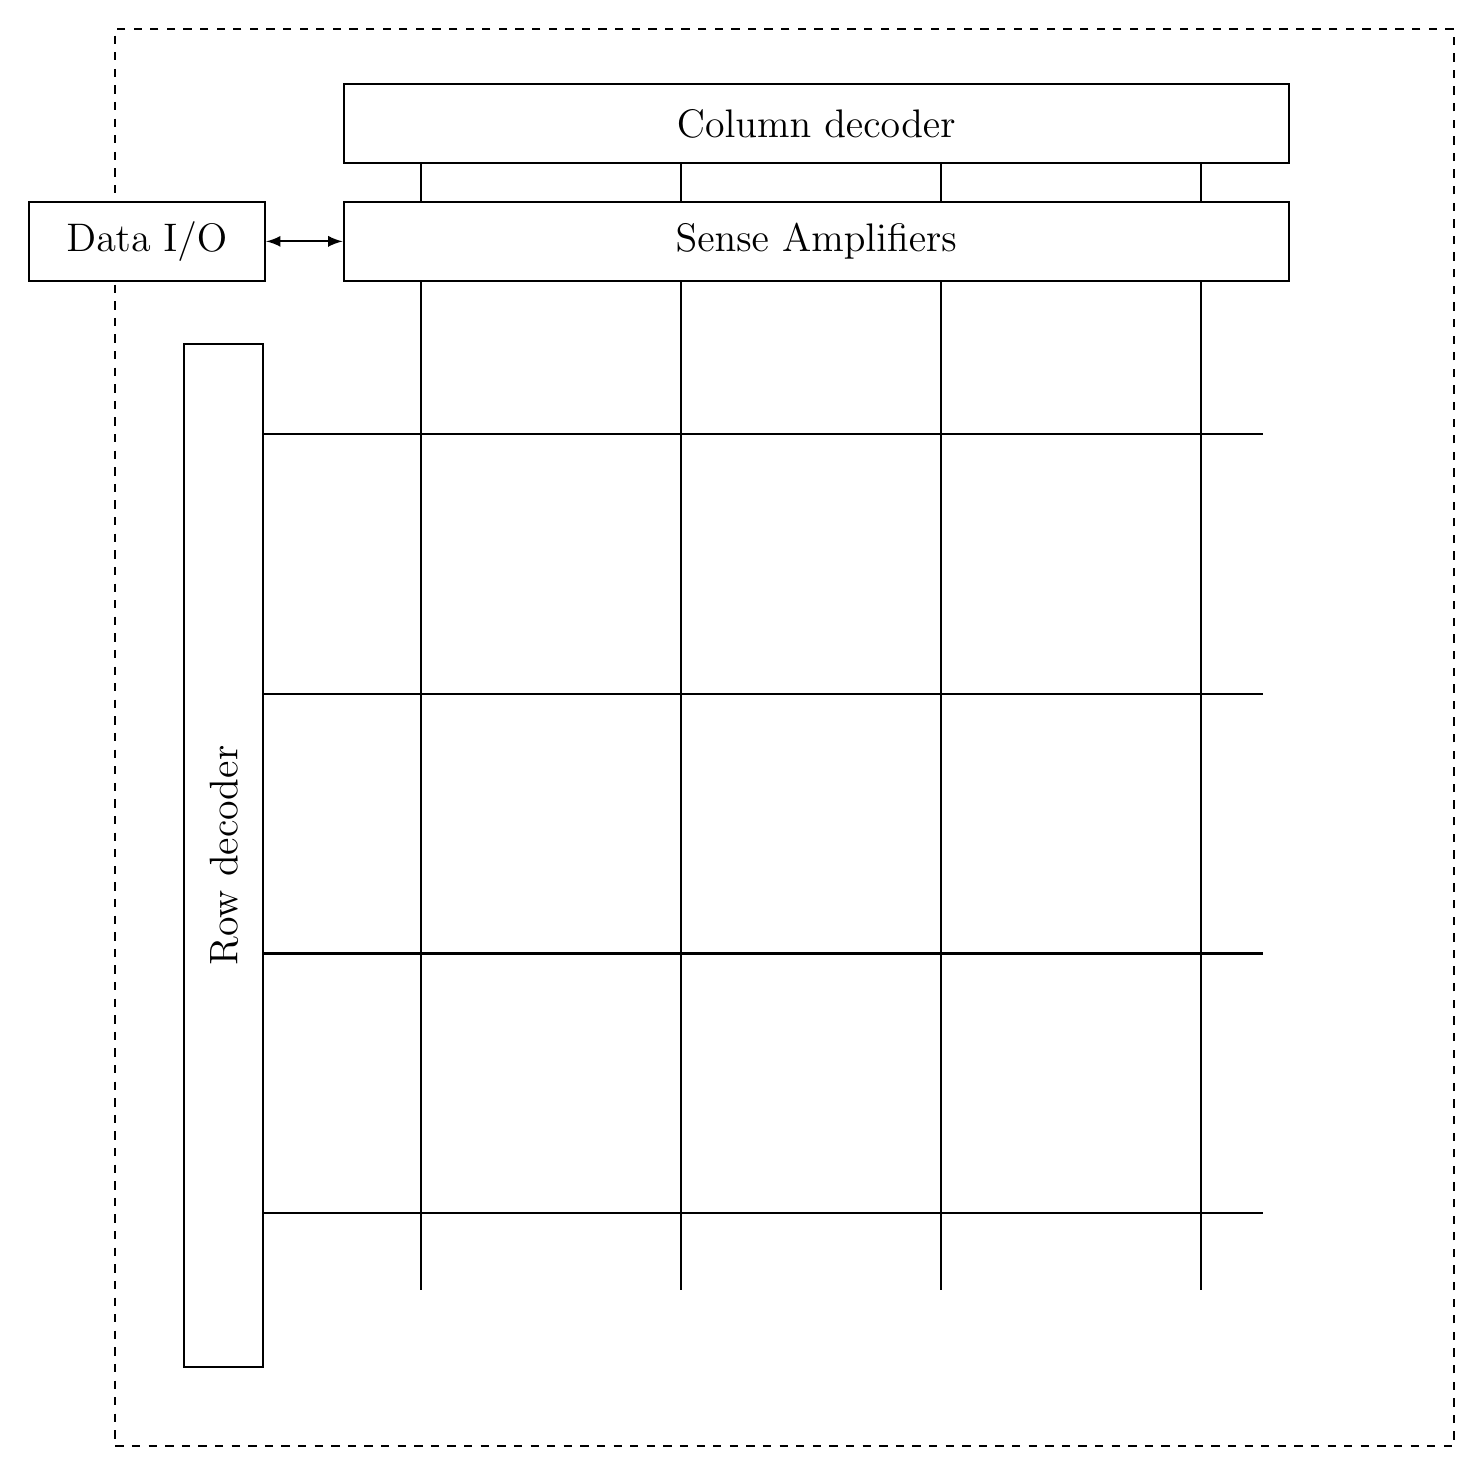
\begin{tikzpicture}[font={\fontsize{15pt}{12}\selectfont}]
    \ctikzset{bipoles/length=1cm}
    
    % Grid of cells
    \dramcell{0}{0}
    \dramcell{0}{3.3}
    \dramcell{0}{6.6}
    \dramcell{0}{9.9}
    \dramcell{3.3}{0}
    \dramcell{3.3}{3.3}
    \dramcell{3.3}{6.6}
    \dramcell{3.3}{9.9}
    \dramcell{6.6}{0}
    \dramcell{6.6}{3.3}
    \dramcell{6.6}{6.6}
    \dramcell{6.6}{9.9}
    \dramcell{9.9}{0}
    \dramcell{9.9}{3.3}
    \dramcell{9.9}{6.6}
    \dramcell{9.9}{9.9}

    % Horizontal wires
    \draw[thick] (-2,0.97) -- (10.685,0.97);
    \draw[thick] (-2,4.27) -- (10.685,4.27);
    \draw[thick] (-2,7.57) -- (10.685,7.57);
    \draw[thick] (-2,10.87) -- (10.685,10.87);

    % Vertical wires
    \draw[thick] (0,0) -- (0,14.3);
    \draw[thick] (3.3,0) -- (3.3,14.3);
    \draw[thick] (6.6,0) -- (6.6,14.3);
    \draw[thick] (9.9,0) -- (9.9,14.3);

    % Big bordering square
    \node[rectangle, draw, color=black, thick, anchor=south west, minimum width=17cm, minimum height=18cm, dashed] at (-3.9,-2) {};

    % Other elements
    \node[rectangle, draw, color=black, thick, anchor=south west, minimum width=12cm, minimum height=1cm, fill=white] (senseamp) at (-1,12.8) {Sense Amplifiers};
    
    \node[rectangle, draw, color=black, thick, anchor=south west, minimum width=12cm, minimum height=1cm] (coldec) at (-1,14.3) {Column decoder} ;
    
    \node[rectangle, draw, color=black, thick, anchor=south west, minimum width=13cm, minimum height=1cm, rotate=90] (rowdec) at (-2,-1) {Row decoder};

    \node[rectangle, draw, color=black, thick, anchor=south west, minimum width=3cm, minimum height=1cm, fill=white] (dataio) at (-5,12.8) {Data I/O};

    \draw[<->, >=latex, thick] (dataio.east) -- (senseamp.west);

\end{tikzpicture}
}
    \caption{Architecture of a DRAM bank.}
    \label{fig_stateOfTheArt_DRAM}
\end{figure}

In order to manage this complexity, the DRAM chips obey to \emph{commands} that
are sent to them by a master \emph{DRAM controller}. For example, in order to
access a specific memory address, the DRAM controller will issue a complex
sequence of commands to connect the sense amplifiers to the correct row with
\emph{Activate} (or \emph{ACT}) and \emph{Precharge} (or \emph{PRE}) commands
and to operate on the specific column using \emph{Read} (or \emph{RD}) or
\emph{Write} (or \emph{WR}) commands.
Figure~\ref{fig_stateOfTheArt_DRAMstateMachine} depicts the possible sequences
of commands that can be issued to a DRAM bank.

In addition to the RD, WR, ACT and PRE, the controller must periodically issue
\emph{Refresh} (or \emph{REF}) commands to avoid the corruption of data.
Indeed, the capacitive nature of DRAM cells is subject to \emph{leakage
current} which deteriorates the voltage stored in the capacitors. The voltages
are kept clearly identifiable as a logical 0 or 1 by \emph{refreshing} the
capacitors' voltages fast enough to never enter an indistinguishable 0 or 1
state. 

\begin{figure}
    \centering
    \scalebox{0.8}{
\begin{tikzpicture}[font={\fontsize{10pt}{12}\selectfont}]

\draw (0,0) node[circle, draw, minimum size=1.8cm] (idle) {Idle};
\draw (4,0) node[circle, draw, text width=1cm, align=center, minimum size=1.8cm] (refresh) {Refre- \\ shing};
\draw (0,-3) node[circle, draw, text width=1cm, align=center, minimum size=1.8cm] (active) {Active \\ row};
\draw (4,-6) node[circle, draw, minimum size=1.8cm] (writing) {Writing};
\draw (-4,-6) node[circle, draw, minimum size=1.8cm] (reading) {Reading};
\draw (0,-9) node[circle, draw, text width=1cm, align=center, minimum size=1.8cm] (precharge) {Pre- \\ charge};

\draw (idle.-25) edge[-latex, thick] node[midway, edgelabel] {REF} (refresh.-155) ;
\draw[->, >=latex, thick, dashed] (refresh.155) -- (idle.25) ;

\draw (idle.south) edge[-latex, thick] node[edgelabel] {ACT}  (active.north) ;

\draw (active.south) edge[-latex, thick] node[near start, edgelabel] {PRE} (precharge.north) ;

\draw (active.east) edge[-latex, thick] node[midway, edgelabel] {WR}  (writing.north) ;
\draw[->, >=latex, thick, dashed] (writing.135) -- (active.-45) ;

\draw (active.west) edge[-latex, thick] node[midway, edgelabel] {RD} (reading.north) ;
\draw[->, >=latex, thick, dashed] (reading.45) -- (active.-135) ;

\draw (reading.-25) edge[-latex, thick] node[near start, edgelabel] {WR} (writing.-155) ;
\draw (writing.155) edge[-latex, thick] node[near start, edgelabel] {RD} (reading.25) ;


\draw (reading.south) edge[-latex, thick] node[midway, edgelabel] {PRE} (precharge.west) ;
\draw (writing.south) edge[-latex, thick] node[midway, edgelabel] {PRE} (precharge.east) ;

\draw[->, >=latex, thick, dashed] (precharge.south) |- (7,-10.5) |- (0,1.5) -- (idle.north);

\draw (reading) edge[loop left, ->, >=latex, thick] node[very near end, edgelabel] {RD} (reading) ;
\draw (writing) edge[loop right, ->, >=latex, thick] node[very near end, edgelabel] {WR} (writing) ;

% Legend
\draw[->, >=latex, thick] (-5.5,0) -- (-4.5,0) node[anchor=west, text width=1cm, align=left] {Command \\ Sequence};
\draw[->, >=latex, thick, dashed] (-5.5,-1) -- (-4.5,-1) node[anchor=west, text width=1cm, align=left] {Automatic \\ Sequence};

\end{tikzpicture}
}
    \caption{Simplified state machine of a DRAM bank access protocol.}
    \label{fig_stateOfTheArt_DRAMstateMachine}
\end{figure}

For physical reasons, complex timing constraints are imposed on a series of
consecutive commands to ensure the correct functioning of a DRAM system. These
constraints (detailed in the JEDEC standard~\cite{JEDEC2012}) must be respected
by the DRAM controller at runtime. Assuming legal sequences~\footnote{By legal
sequences, we mean sequences that respect the state machine of
Figure~\ref{fig_stateOfTheArt_DRAMstateMachine}.} of commands, we provide to
the reader an overview of the major timing constraints that can be found in the
JEDEC standard.

\begin{itemize}
    \item[\textbf{ACT}] The row activate command is associated to four major
        timing constraints:
        \begin{itemize}
            \item[$t_{RCD}$] Row to Column Delay. This parameter represents the
                time physically required to connect the sense amplifier to the
                row. The memory controller must wait during at least $t_{RCD}$
                cycles after the ACT before it can issue a RD or a WR.
            \item[$t_{RAS}$] Row Access Strobe. When the sense amplifiers are
                connected to a row, they slightly modify the voltage of the
                storage capacitors of the cells. So, just after the connection,
                the sense amplifiers \emph{restore} the voltages of the
                capacitors in order to avoid any corruption on the data.
                $t_{RAS}$ is the time required by the sense amplifiers for this
                restoration. For this reason, $t_{RAS}$ is the minimum time a
                row must remain opened before it can be precharged.
            \item[$t_{RRD}$] Row activate to Row activate Delay. It is the
                minimum time required between two $ACT$ commands. This allows
                to limit peak current.
            \item[$t_{FAW}$] Four row Activation Window. It is a sliding window
                during which no more than 4 $ACT$ commands can be issued in
                order to limit peak current.
        \end{itemize}
    
    \item[\textbf{PRE}] The precharge command is associated to two major timing
        constraints:
        \begin{itemize}
            \item[$t_{RP}$] Row Precharge delay. It is the time required to
                disconnect from the current row and reset the sense amplifiers
                to a neutral voltage level.
            \item[$t_{RC}$] Row Cycle. $t_{RC} = t_{RAS} + t_{RP}$ is a
                commonly used indicator for DDR SDRAM performance as it is the
                minimum time allowed between two $ACT$ can be issued to the
                same bank.
        \end{itemize}

    \item[\textbf{RD}] The read command is associated to two major timing
        constraints:
        \begin{itemize}
            \item[$t_{CAS}$] Column Access Strobe. It is the duration required
                by the memory to place on the data bus the requested data. This
                parameter is also often noted $t_{CL}$.
            \item[$t_{burst}$]  It is the time (in cycles) required to transfer
                a complete burst. If the memory data bus is $w_{bus}$ bytes
                large, a complete burst will be transferred in
                ${s_{burst}}/{w_{bus}}$ beats of data. In DDR SDRAM systems,
                the double data rate mechanism allows to transfer two beats of
                data by cycle. So, $t_{burst} = {s_{burst}}/(2 \times w_{bus})$
                cycles.
        \end{itemize}
    
    \item[\textbf{WR}] The Write command is associated to four major timing
        constraints
        \begin{itemize}
            \item[$t_{burst}$] Same as RD.
            \item[$t_{CWD}$] Column Write Delay. Delay between the $WR$ command
                and the placement of data on the bus.
            \item[$t_{WTR}$] Write To Read delay. Minimum time between a $WR$
                and a $RD$ command. This constraint is related to the bus
                switching time. $t_{WTR}$ is not local to a bank but a global
                device constraint.
            \item[$t_{WR}$] Write Recovery delay. This is the time between the
                end of the data burst and the complete propagation of the data
                in the DRAM array. So, $t_{WR}$ is the minimum amount of time
                to wait after a column write command before a precharge command
                can be issued.
        \end{itemize}
    
    \item[\textbf{REF}] The Refresh command is associated to two major timing
        constraints:
        \begin{itemize}
            \item[$t_{REFI}$] Refresh interval. It is the time between two
                $REF$ commands issued by the controller. So, $t_{REFI} =
                T_{refresh} / N_{refresh}$ (usually $7.8\mu$s  or $3.9\mu$s
                depending on the operating temperature). 
            \item[$t_{RFC}$] Refresh Cycle. It is the time required to refresh
                $N_{row}^{ref}$ rows. This parameter depends on the memory
                density. It can be (over-)approximated by $N_{row}^{ref} \times
                t_{RC}$.\\
        \end{itemize}
\end{itemize}

In order to give to the reader the order of magnitude of each previously
enumerated timing parameters, we provide in
table~\ref{table_stateOfTheArt_exampleTimingParamsMicronDRAM} an example of
timing constraints extracted from the documentation of a Micron DDR3-SDRAM
module~\cite{Doc_micron}.

\begin{table}
\begin{center}
    \begin{tabular*}{0.8\linewidth}{@{\extracolsep{\fill}} c c c c}
	\hline
	Parameter 	& Nanoseconds	& Cycles	& Data beats 	\\
	\hline
	$t_{CK}$ 	& 1.25		& 1 		& 2  		\\
	$t_{BURST}$ & 5         & 4         & 8  		\\ 
	$t_{CAS}$ 	& 13.75		& 11 		& 22 		\\ 
	$t_{RP}$ 	& 13.75		& 11 		& 22 		\\ 
	$t_{RCD}$ 	& 13.75		& 11 		& 22 		\\ 
	$t_{WR}$ 	& 21.25		& 17 		& 34 		\\ 
	$t_{WTR}$ 	& 7.5 		& 6 		& 12 		\\ 
	$t_{RAS}$ 	& 35		& 28 		& 56 		\\ 
	$t_{RC}$ 	& 48.75		& 39 		& 78 		\\ 
	$t_{FAW}$ 	& 30		& 24 		& 48 		\\ 
	$t_{RRD}$ 	& 6.25 		& 5 		& 10 		\\ 
	$t_{CWD}$ 	& 10		& 8 		& 16 		\\ 
	$t_{RFC}$ 	& 260		& 208 		& 416 		\\
	$t_{REFI}$  & 3906		& 3125 		& 6250 		\\ 
	\hline	
\end{tabular*}
\end{center}
%\caption{Timing parameters of Micron module \cite{Doc_micron}}
\caption{Example of timing constraints extracted from the Micron 4GB
    MT41K512M8-125 DDR3 SDRAM module documentation~\cite{Doc_micron}.}
\label{table_stateOfTheArt_exampleTimingParamsMicronDRAM}
\end{table}

The sense amplifiers are commonly seen as \emph{row-buffers}\footnote{Also
denoted as the \emph{row caches} in some papers}, in which requests can be
issued efficiently. Similarly to classical caches, the memory requests can thus
be classified as \emph{row hits} when the targeted data is present into the
row-buffer or \emph{row-misses} when the request targets a closed row. In
modern DRAM controller, the management of such row buffers usually implements
one of the two following policies:
\begin{itemize}
    \item \emph{open-page}: \emph{PRE} commands are issued only in case of a
        row-miss of a refresh, thus exploiting the spatial and temporal
        locality principle. In general, the open-page policy performs best with
        high row-hit ratios.
    \item \emph{close-page}: every \emph{RD} or \emph{WR} command is
        systematically followed by a \emph{PRE} command. This performs best
        under high row-miss ratios when accesses mostly target random locations
        in memory.
\end{itemize}

\begin{example}[Row-buffer management policies]
    \label{ex_stateOfTheArt_rowBufferManagementPolicy}
    Table~\ref{table_stateOfTheArt_exampleOpenClosePageDRAM} shows an example
    of six memory requests and the associated sequences of commands in
    open-page and close-page row-buffer management policies. The
    Figure~\ref{fig_stateOfTheArt_DRAMchronogram} shows the time diagram of
    commands with the associated timing constraints.
    \begin{table}
        \begin{center}
            \begin{tabular*}{1\linewidth}{@{\extracolsep{\fill}} c c c c | l l}
            \hline
                \multicolumn{4}{c|}{\sc Input request} & \multicolumn{2}{c}{\sc Generated commands} \\
            \hline
                Req. no. & Type & Bank & Row & Open-page & Close-page\\
            \hline
                1 & Read & 1 & 1 & \emph{ACT - RD} & \emph{ACT - RD - PRE}\\
                2 & Read & 1 & 1 & \emph{RD} &  \emph{ACT - RD - PRE}\\
                3 & Read & 1 & 1 & \emph{RD} &  \emph{ACT - RD - PRE}\\
                4 & Write & 1 & 2 & \emph{PRE - ACT - WR} &  \emph{ACT - WR - PRE}\\
                5 & Read & 2 & 1 & \emph{ACT - RD} &  \emph{ACT - RD - PRE}\\
                6 & Read & 1 & 1 & \emph{PRE - ACT - RD} &  \emph{ACT - RD - PRE}\\
            \hline
            \end{tabular*}
        \end{center}
        \caption{Example of DRAM commands issued under open-page and close-page
            row-buffer management policies}
        \label{table_stateOfTheArt_exampleOpenClosePageDRAM}
    \end{table}

    \begin{figure}
        \centering
        \tikzset{timing/.append style={x=1.2ex, y=2.3ex}}
        \rotatebox{90}{
\begin{tikztimingtable}[timing/coldist=0.5, timing/d/text/.append style={font=\rmfamily}, timing/d/background/.style={fill=white}]
    {\rmfamily CLK} &  10{0.5C} M 62{0.5C} M 16{0.5C} M 22{0.5C} M 24{0.5C} M 10{0.5C} M 12{0.5C}\\
    {\rmfamily CMD} &  U 3D{ACT}     UMU   3D{RD}   U 3D{RD}   U 3D{RD}      15U 3D{PRE}     UMU  3D{ACT}    3D{ACT}    UMU  3D{WR}    3U 3D{RD}      UMU  4U         3U 3D{PRE}    UMU 3D{ACT}    UMU  4U U\\
    {\rmfamily ADDR} & U 3D{B1.R1}   UMU   3D{B1.R1} U 3D{B1.R1} U 3D{B1.R1} 15U 3D{B1.R1}   UMU  3D{B1.R2}  3D{B2.R1}  UMU  3D{B1.R2} 3U 3D{B2.R1}   UMU  4U         3U 3D{B1.R2}  UMU 3D{B1.R1}  UMU  4U U\\
    {\rmfamily DATA} & U 3U          UMU   3U 11U  4D{Req.1} 4D{Req.2} 4D{Req.3} 3U          UMU  3U         3U         UMU  3U        4D{Req. 4} 2U  UMU  4D{Req. 5} 3U 3U         UMU 3U         UMU  4D{Req. 6} U\\
\extracode

\Cote[-5mm]{(4,-6)}{(10,-6)}{ \tiny $t_{RCD}$ }<h>
\Cote[-5mm]{(10,-6)}{(14,-6)}{ \tiny $t_{bst}$ }<h>
\Cote[-10mm]{(10,-6)}{(21,-6)}{ \tiny $t_{CAS}$ }<h>
\Cote[-5mm]{(21,-6)}{(25,-6)}{ \tiny $t_{bst}$ }<h>
\Cote[-5mm]{(25,-6)}{(29,-6)}{ \tiny $t_{bst}$ }<h>
\Cote[-5mm]{(29,-6)}{(33,-6)}{ \tiny $t_{bst}$ }<h>

\Cote[-5mm]{(36,-6)}{(42,-6)}{ \tiny $t_{RP}$ }<h>
\Cote[-5mm]{(42,-6)}{(51,-6)}{ \tiny $t_{RCD}$ }<h>
%\Cote[-5mm]{(51,-6)}{(55,-6)}{ \tiny $t_{bst}$ }<h>
\Cote[-10mm]{(48,-6)}{(54,-6)}{ \tiny $t_{WTR}$ }<h>

%\Cote[-5mm]{(57,-6)}{(60,-6)}{ \tiny $t_{CAS}$ }<h>
\Cote[-5mm]{(60,-6)}{(64,-6)}{ \tiny $t_{bst}$ }<h>

\Cote[-10mm]{(55,-6)}{(70,-6)}{ \tiny $t_{WR}$ }<h>

\Cote[-5mm]{(70,-6)}{(76,-6)}{ \tiny $t_{RP}$ }<h>

\Cote[-5mm]{(79,-6)}{(83,-6)}{ \tiny $t_{bst}$ }<h>

\begin{background}
    \vertlines[dashed]{}
\end{background}
\end{tikztimingtable}


}
        \caption{DRAM commands under open-page row-buffer management policies for
            requests of example~\ref{ex_stateOfTheArt_rowBufferManagementPolicy} }
        \label{fig_stateOfTheArt_DRAMchronogram}
    \end{figure}
\end{example}


Finding a tight upper-bound on the time required to read or write a data
from/to a COTS DRAM system can be challenging because of the complexity of its
access protocol. Indeed, the time required to access a data highly depends on
the current DRAM state and is thus strongly dependent on the history of
requests. Moreover, modern multi and many-core processors usually feature
several components able of addressing the DRAM directly. However, the DRAM
controller still answers a series of requests that results from the arbitration
of the concurrent accesses. The performance of the DRAM subsystem in a multi or
many-core context is thus strongly correlated to the ability of the arbiter to
issue the requests in a \emph{favorable} order that will enable to hide most of
the JEDEC timing constraints thank to pipelining effects. \\

In the next section, we will analyze the methods that have been proposed to
compute bounds on the \emph{Worst-Case Traversal Time} of NoC packets and the
DDR-SDRAM access durations.



\section{Interference penalties on many-core processors}
\label{sec_stateOfTheArt_interferencePenalties}

Time-compositional approaches enable decoupled analysis of the program
execution and the interferences on shared resources. Yet, the underlying
assumption when applying such methods is that analyzing the shared resources
interferences is possible. In this section, we overview the state-of-the-art
methods for computing bounds on interference penalties when accessing NoCs and
DRAM subsystems.

\subsection{Network on Chip}
\label{sssec_stateOfTheArt_Noc_timingguarantees}

\subsubsection{Deadlocks}
\label{sssec_stateOfTheArt_Noc_deadlocks}
In wormhole switched networks, one message can be holding one resource while
requesting others, and thus, cause a deadlock~\cite{Duato1993, Fleury98}. The
avoidance of deadlock is a major problem that must be solved before any of the
WCTT estimation techniques that will be presented below can be applied.

\begin{example}[Deadlock on a wormhole-switched NoC]
    \begin{figure}
        \centering
        \scalebox{0.5}{
% #1 x, #2 y, #3 no, #4-6 text
\newcommand\nocswitchbuffertxt[6]{
    \draw (#1, #2) node[draw, thick, minimum width=2.5cm, minimum height=0.8cm, anchor=north, inner sep=0pt] (s1#3) {#6};
    \draw (#1, #2 + 0.8) node[draw, thick, minimum width=2.5cm, minimum height=0.8cm, anchor=north, inner sep=0pt] (s2#3) {#5};
    \draw (#1, #2 + 1.6) node[draw, thick, minimum width=2.5cm, minimum height=0.8cm, anchor=north, inner sep=0pt] (s3#3) {#4};
    \draw[thick] ([xshift=0.04em]s1#3.south west) -- ([xshift=0.04em, yshift=-1em]s1#3.south west);
    \draw[thick] ([xshift=-0.04em]s1#3.south east) -- ([xshift=-0.04em, yshift=-1em]s1#3.south east);
}

% #1 x, #2 y, #3 no, #4-6 text
\newcommand\nocnode[4]{
    \draw (#1,#2) node[draw, circle, thick, minimum size=1.1cm, inner sep=0pt] (#3) {#4};
}
% #1 x, #2 y, #3 no
\newcommand\nocnodestop[3]{
    \draw (#1,#2) node[draw, circle, thick, fill=black, minimum size=0.15cm, inner sep=0pt] (#3) {};
}

\begin{tikzpicture}[font={\fontsize{15pt}{12}\selectfont}]
\nocnode{0}{0}{r1}{$R_1$}
\nocnode{-8}{0}{r2}{$R_2$}
\nocnode{-8}{8}{r3}{$R_3$}
\nocnode{0}{8}{r4}{$R_4$}

\nocnodestop{0}{1.2}{stopr1}
\nocnodestop{-6.8}{0}{stopr2}
\nocnodestop{-8}{6.8}{stopr3}
\nocnodestop{-1.2}{8}{stopr4}

\nocswitchbuffertxt{-8}{-4}{sr2}{$F(R_4)$}{}{}
\nocswitchbuffertxt{-8}{4}{sr3}{$F(R_4)$}{$F(R_4)$}{$F(R_4)$}

\begin{scope}[rotate=-90, transform shape]
\nocswitchbuffertxt{-8}{-12}{wr3}{$F(R_1)$}{}{}
\nocswitchbuffertxt{-8}{-4}{wr4}{$F(R_1)$}{$F(R_1)$}{$F(R_1)$}
\end{scope}

\begin{scope}[rotate=90, transform shape]
\nocswitchbuffertxt{0}{-4}{er1}{$F(R_3)$}{}{}
\nocswitchbuffertxt{0}{4}{er2}{$F(R_3)$}{$F(R_3)$}{$F(R_3)$}
\end{scope}

\begin{scope}[rotate=180, transform shape]
\nocswitchbuffertxt{0}{-12}{nr4}{\rotatebox{180}{$F(R_2)$}}{}{}
\nocswitchbuffertxt{0}{-4}{nr1}{\rotatebox{180}{$F(R_2)$}}{\rotatebox{180}{$F(R_2)$}}{\rotatebox{180}{$F(R_2)$}}
\end{scope}


\draw[thick, ->, >=latex] (s3sr2.north) -- (r2.south); 
\draw[thick, ->, >=latex] (s3wr3.north) -- (r3.west); 
\draw[thick, ->, >=latex] (s3nr4.north) -- (r4.north); 
\draw[thick, ->, >=latex] (s3er1.north) -- (r1.east); 

\draw[thick, ->, >=latex] (r2.north) -- (s1sr3.south); 
\draw[thick, ->, >=latex] (r3.east) -- (s1wr4.south); 
\draw[thick, ->, >=latex] (r4.south) -- (s1nr1.south); 
\draw[thick, ->, >=latex] (r1.west) -- (s1er2.south); 

\draw[thick, dashed] (s3nr1.north) -- (stopr1); 
\draw[thick, dashed] (s3er2.north) -- (stopr2); 
\draw[thick, dashed] (s3sr3.north) -- (stopr3); 
\draw[thick, dashed] (s3wr4.north) -- (stopr4); 

 
\end{tikzpicture}
}
        \caption{Example of deadlock on a wormhole-switched NoC.}
        \label{fig_stateOfTheArt_NoCdeadlock}
    \end{figure}
    Figure~\ref{fig_stateOfTheArt_NoCdeadlock} depicts an example of deadlock
    in a wormhole-switched network. We can see the flits $F(R_X)$ of 4 packets
    in the FIFO queues of the interfaces of 4 routers. 3 out of 4 flits
    $F(R_1)$ at destination of the router $R_1$ went through the router $R_3$
    and are stored in one queue of the router $R_4$ waiting for availability of
    the link to $R_1$. Because of the back-pressure mechanism, the fourth
    $F(R_1)$ flit is still queueing in $R_3$ as the queue of $R_4$ is full. It
    is also maintaining occupied the link between $R_3$ and $R_4$ as all the
    flits of one packet must be consecutive. At the same time, the flits
    $F(R_2)$ blocking the flits $F(R_1)$ are waiting for the link between $R_1$
    and $R_2$ to become idle. Similarly, the flits $F(R_3)$ occupying this link
    are waiting for the link between $R_2$ and $R_3$ to become idle but this
    link is occupied by the $F(R_4)$ flits themselves waiting for the $R_3$ to
    $R_4$ link that is occupied by the $F(R_1)$ flits. We can see clearly here
    the occurrence of an unsolvable cyclic dependency leading to a deadlock. In
    this case, the time needed by a packet to cross the network cannot be
    bounded. 
\end{example}

Different approaches have been proposed in order to tackle the problem of
deadlocks. In~\cite{Dally1987}, Dally \etal provided a method to construct
deadlock-free \emph{non-adaptive} routing algorithms. They pointed out the
correlation between deadlocks and the presence of cycles in the \emph{Channel
Dependency Graph} (or \emph{CDG}) which represents the connections for all
pairs of communication channels. They demonstrate that a routing algorithm is
deadlock-free if and only if it produces CDG without cycles and they provide a
method for breaking the cycles in a CDG using the notion of \emph{Virtual
Channel}. \\

In~\cite{Duato1993}, Duato extended the work of Dally \etal and developed a
theoretical framework for the design of deadlock-free \emph{adaptive} routing
algorithms for wormhole-switched networks. He demonstrated that the absence of
cycles in the CDG is not required to construct adaptive deadlock-free routing
algorithms and, based on that, he proved that, in this case, only the absence
of cycles in the extended channel dependency graph of a routing sub-function is
required. In~\cite{Duato1995}, he extended his results to more general class of
adaptive routing algorithms. \\

Many additional contributions have been proposed to tackle the problem of
deadlock avoidance in wormhole switched networks~\cite{Jayasimha2003, Lin1991,
Schwiebert1995}. In~\cite{Fleury98}, Fleury \& Fraigniaud proposed a unified
definition of a routing function that captures most of the already existing
definitions of the literature and extend their work to treat the problem of
multicast routing algorithms. \\

In~\cite{Dinechin2014NoCArc}, Dupont de Dinechin \etal proposed a different
solution to the deadlock avoidance problem on the \mppalong. They use the
hardware limiters of the NoC interfaces in order to regulate the traffic
injected on the network. By doing so, they are able to bound the maximum
possible backlog for all the routers' buffers and they show that, assuming a
proper configuration of the HW limiters, no buffer ever overflows, thus
avoiding any potential deadlock.\\



\subsubsection{Computing WCTT with Network Calculus}

In a hard-real time context, the estimation of the WCTT of a NoC packet is
commonly achieved using \emph{Network Calculus}~\cite{LeBoudec2001, Cruz91} or
\emph{Real-time calculus}~\cite{Thiele2000}. In either cases, the deadlock
problem is usually assumed to be solved before the application of the
technique.


The term of \emph{Network Calculus} (or \emph{NC}) refers to a collection of
mathematical results used for the modeling and the analysis of deterministic
queueing systems thanks to \emph{Min-Plus} algebra. Using NC, the communication
flows are modeled as cumulative functions counting the amount of data injected
in the network over time. The traffic of all communication flows is assumed to
be limited at source. The maximum envelope of traffic allowed for a
communication flow is represented by the concept of an \emph{arrival curve}.

\begin{definition}[Arrival curve]
    An arrival curve $\alpha(t)$ is said to constrain a cumulative flow $x(t)$
    if it verifies the relation~\ref{eq_stateOfTheArt_arrivalCurve}.
    \begin{equation}
        \label{eq_stateOfTheArt_arrivalCurve}
        \forall s \leq t, \;  x(t) - x(s) \leq \alpha(t-s)
    \end{equation}
    Thanks to the Min-plus convolution denoted $\otimes$, the
    equation~\ref{eq_stateOfTheArt_arrivalCurve} can be rewritten as:
    \begin{displaymath}
        x(t) \leq ( \alpha \otimes x ) (t)
    \end{displaymath}
\end{definition}
The major assumption of NC is that the  injected traffic is constrained by
arrival curves. In return, network nodes are assumed to provide some form of
guaranteed services. The scheduling operated by a network node is modeled under
the notion of \emph{service curve}. 

\begin{definition}[Service curve]
    A network node $\mathcal{N}$ is said to offer a service curve $\beta$ to an
    input flow $x(t)$ if its output flow verifies the
    relation~\ref{eq_stateOfTheArt_serviceCurve}.  \begin{equation}
        \label{eq_stateOfTheArt_serviceCurve}
        \forall t, \exists s \leq t, \; y(t) - x(s) \geq \beta(t-s)
    \end{equation}
    Using Min-plus convolution, equation~\ref{eq_stateOfTheArt_serviceCurve}
    can be rewritten as:

    \begin{displaymath}
        y(t) \geq ( \beta \otimes x ) (t)
    \end{displaymath}
\end{definition}
The succession of network nodes crossed by a flow can be modeled by
concatenating the nodes using the Min-plus convolution of their respective
service curves.
\begin{example}[Concatenation of network nodes]
    Let $\mathcal{N}_1$ and $\mathcal{N}_2$ be two network nodes respectively
    offering the service curves $\beta_1$ and $\beta_2$. Any flow crossing
    $\mathcal{N}_1$ and $\mathcal{N}_2$ consecutively is offered the service
    curve $\beta_1 \otimes \beta_2$
\end{example}
Based on these models, NC helps in computing safe bound on the maximum
\emph{backlog} of each network node which represents the maximum amount of
buffered data in a network switch. The backlog of a network node is defined as
the difference between its input and output flow, i.e, $x(t) - y(t)$.
Equation~\ref{eq_stateOftheArt_NCbacklog} is classical NC result providing a
bound on the backlog.

\begin{equation}
    \label{eq_stateOftheArt_NCbacklog}
    x(y) - y(t) \leq \underset{s \geq 0}{\text{sup}} \{ \alpha (s) - \beta (s) \}
\end{equation}
If the backlog never overpasses the size of the switch's buffers, then it is
sound to assume that no buffer will overflow. Similarly, NC provides
upper-bounds on the maximum \emph{delay} suffered by a flow crossing the
network. Let $\Delta (s) = inf \{ \tau \geq 0 \; : \; \alpha (s) \leq \beta ( s
+ \tau )\}$ be the virtual delay of a system having $\alpha$ as input and
$\beta$ as output, let $h( \alpha , \beta )$ be the supremum of all values of
$\delta (s)$, the delay $d(t)$ is given by
Equation~\ref{eq_stateOftheArt_NCdelay}.

\begin{equation}
    \label{eq_stateOftheArt_NCdelay}
    d(t)  \leq h( \alpha , \beta )
\end{equation}
Figure~\ref{fig_stateOfTheArt_NCcumulCurves} shows two cumulative function
representing an input flow $x(t)$ and an output flow  $y(t)$ with a graphical
representation of the backlog (\tikz{\draw[latex-latex, densely dotted, thick]
(0.0,0.5) -- (0.7,0.5);}) and delay (\tikz{\draw[latex-latex, dashed, thick]
(0.0,0.5) -- (0.7,0.5);})functions.

\begin{figure}
    \centering
    \scalebox{1.3}{
\pgfplotstableread{imgs/tex/dat/stateOfTheArt_cumulCurves.dat}\stateoftheartCumulCurvesdat
%\pgfplotstableread{dat/stateOfTheArt_cumulCurves.dat}\stateoftheartCumulCurvesdat
\begin{tikzpicture}
    \begin{axis}[
        xmin=0,
        xmax=10,
        ymin=0,
        ymax=5.5,
        xticklabels={ },
        yticklabels={ },
        axis x line=middle,
        axis y line=middle,
        ylabel = {\scriptsize Cumulative data amount},
        y label style={at={(axis description cs:-0.02,.5)},rotate=90,anchor=south},
        xlabel = {\scriptsize Time},
        x label style={at={(axis description cs:0.5,-0.04)},anchor=north},
        ticks=none,
        width=10cm,
        height=5cm
        ]
        \addplot[mark=none, thick] table[x index=0, y index=1]{\stateoftheartCumulCurvesdat};
        \addplot[mark=none, thick ] table[x index=0, y index=2]{\stateoftheartCumulCurvesdat};
    \end{axis}
    \draw[latex-latex, dashed, thick] (2.1, 1.2) -- (5.7, 1.2) node [very near end, above] {\scriptsize $d(t)$};
    \draw[latex-latex, densely dotted, thick] (3.7, 0.25) -- (3.7, 1.55) node [very near start, left] {\scriptsize $x(t) - y(t)$};

    \draw (7.1,2.1) node {\scriptsize $y(t)$};
    \draw (5.1,2.7) node {\scriptsize $x(t)$};
\end{tikzpicture}
}
    \caption{Example of two cumulative flows with graphical representation of
    the backlog and the delay}
    \label{fig_stateOfTheArt_NCcumulCurves}
\end{figure}


Qian \etal~\cite{Qian2009, Qian2010} and Zhan \etal~\cite{Zhan2013}
demonstrated the effectiveness of Network Calculus on NoCs, which was mostly
used for the timing analysis of macroscopic-sized networks beforehand. Since
then, NC has then been successfully applied to NoCs several times and notably
on the \mppalong in~\cite{Dinechin2014} and~\cite{Giannopoulou2015}. \\

Dupont de Dinechin \etal~\cite{Dinechin2014} used the work of
Cruz~\cite{Cruz91} and Zhang~\cite{Zhang1995} on $(\rho , \sigma)$ calculus to
derive backlog and delay bounds on the \mppalong. They derived from the main
$(\rho , \sigma)$ relations a quadratic optimization problem whose solutions
can be transcribed into configurations of the hardware limiters featured by the
\mppalong's NoC interfaces. Giannopoulou \etal proposed
in~\cite{Giannopoulou2015} a similar method to compute $(\rho , \sigma)$
parameters of the \mppalong's hardware limiters based on backlog and delay
constraints and they extended the approach to bound the number of memory
accesses performed during the reception of NoC packets in a pre-definite time
frame. \\

In this section, we focused on WCTT estimation for NoCs and, in particular, on
the classical methods for avoiding deadlocks and the application of Network
Calculus. In general, the WCET of tasks busy-waiting for packet reception must
be computed with the addition of stalling timing penalties depending on the
WCTT. This means that the WCET of such task is computed with timing penalties
that are functions of the packets' WCTTs. Thus, the temporal validation of
programs as required by certification depends not only on the WCETs of tasks
but also on the WCTTs of packets sent through the NoC. Consequently, management
of NoC sharing appears as a major issue for predictability. \\


In addition to the NoC, it appears that many-core architectures can also put
high pressure on memory subsystems since the number of cores composing the
processor can be high. Serving memory requests from many cores requires a high
throughput. When such a resource is massively shared, being able to provide
tight timing guarantees to applications can become challenging. The
state-of-the-art methods that were proposed to upper-bound the duration of
DDR-SDRAM transactions are overviewed in the next section.  



\subsection{Temporal bound for DRAM subsystems}
Several works have already been carried-out to bound memory access durations of
existing unmodified applications on COTS targets. Usually, they rely on
detailed models of the memory access protocol provided together with a fine
grained analysis of the COTS memory controller. For example, Wu \etal proposed
in~\cite{Wu2013} a worst-case analysis for DDR-SDRAM in multi-core processors
that benefits from an explicit DRAM state model. They assume a global FIFO
queue of size $n$ arbitrating the requests concurrently issued by the $n$
cores. This provides a bounded service time for all requesters. With a similar
approach, Ding \etal analyzed in~\cite{ding2013} the DRAM access protocol with
FIFO arbitration and close-page row-buffer management policy. 

Unfortunately, modern DRAM controllers (such as the arbiter of the \mppalong
detailed in Section~\ref{sssec_systemModel_MPPADRAMarbiter}) usually feature
more complex out-of-order arbiters with open-page row-buffer management policy
enabling better memory throughput in average~\cite{Rixner2000}. The
\emph{First-Ready First-Come First-Serve} (or \emph{FR-FCFS}) arbitration
scheme, which is probably the most widely used in existing COTS processors,
prioritize requests on already opened rows over requests on closed rows no
matter how long they have been pending. So, theoretically, the service time of
a request cannot be bounded because of potential starvation problems. Several
contributions have been proposed to overcome this issue by modeling the whole
the memory hierarchy, including the caches, instead of the DRAM controller's
policy alone. Although not implementing a pure FR-FCFS policy, the \mppalong's
arbiter also prioritize requests on already opened rows over others in the
Reordering pool. Since this behaviour is very comparable to a FR-FCFS arbiter,
the analysis of other works focusing on open-page FR-FCFS controllers appears
to be relevant in our case.\\

In~\cite{kim2014bounding}, Kim \etal tackled the problem of bounding memory
interference delays with a realistic FR-FCFS arbitration policy thanks to three
assumptions on the system model: each task has been allocated a sufficient
space in cache to store a complete DRAM row;  all memory accesses are aligned
with DRAM columns and  tasks do not share memory. The authors propose to use
two different approaches: 1) the \emph{request-driven} approach which
essentially consists in summing the maximum delays involved by each memory
request issued from a task; and 2) the \emph{job-driven} approach where the
delays are derived from the worst interference scenario of co-running tasks.
The authors argue that combining these two approaches enables to compute safe
bounds on the worst case response time of each task in situation of
interference. \\

In~\cite{Yun2015}, Yun \etal extended the analysis of~\cite{kim2014bounding} to
consider modern COTS processors where: 1) each core can issue several
outstanding requests to mask memory latency; 2) the arbitration scheme uses
FR-FCFS with higher priorities for \emph{RD} over \emph{WR} commands; and 3)
\emph{RD} and \emph{WR} commands are issued in \emph{batches} using a classical
watermark mechanism~\cite{Chatterjee2012}. They also assume specific hardware
configurations such as partitioned caches and DRAM banks to limit interferences
by design. \\

The problem of handling refreshes is commonly treated separately from the DRAM
system analysis~\cite{Atanassov2001, Bhat2010, kim2014bounding} by adding to
the memory delay initially computed a refresh penalty $E_R$ defined as the
fixed point of the recursive equation~\ref{eq_stateOfTheArt_DRAMrefresh} with
$E_R^0 = 0$.
\begin{equation}
    \label{eq_stateOfTheArt_DRAMrefresh}
    E_{R}^{k+1} = \left\lceil \frac{ (\text{total delay from analysis}) + E_R^k }{ t_{REFI} } \right\rceil \times t_{RFC}
\end{equation}


On the \mppalong, the accesses to the DDR-SDRAM are not due to cache refills of
evictions. To the best of our knowledge, no already published work consider
many-core processors where memory transactions are achieved using DMA transfers
that are likely to be large and explicitly initiated by software.  Overall,
bounding the WCET of a task accessing the main memory requires to bound the
duration of memory transactions. In a time-compositional approach, the bound on
the memory access duration when interfering with other memory masters can be
used as a timing penalty that is summed to the WCET of the task without
interferences. Despite accurate models, the memory latency bounds provided by
purely analytical approaches are usually driven by a pathological pattern of
requests for which the average-case optimization mechanisms of the controller
performs poorly. As explained in
section~\ref{sec_stateOfTheArt_predictableDesign}, if the bound provided by
these approaches are not sufficient, the issue is usually overcome using either
bespoke DRAM controllers which achieve highly timing-predictable accesses to
memory or appropriate software to avoid pathological situations.


\subsection{End-to-end timing bounds on multiple resources}
Many-core processors have a hierarchical architecture. For this reason, the
interferences on shared resources often appear simultaneously at different
levels. For example, a transaction to the main memory initiated by a core
usually imply potential interferences at both the NoC and the DDR-SDRAM levels.
Hence, the timing behaviour of the two resources are inter-dependent and must
not be considered separately. The end-to-end timing analysis of multi-resource
interferences is thus a major problem to bound execution time many-core
processors. Yet, this problem was mostly unexplored in past contributions.
In~\cite{Perret16}, we provided models of all shared resources on a \mppalong
processor and we proposed an approach to compose the output of these models in
an end-to-end timing analysis of DDR-SDRAM transaction. We will detail this
contribution in Chapter~\ref{chap_execModel}.


\section{Enforcing time-predictability by design}
\label{sec_stateOfTheArt_predictableDesign}

We overviewed in Section~\ref{sec_stateOfTheArt_interferencePenalties} the
methods for computing interference penalties when accessing the NoC and the
DRAM subsystem on a many-core processor. Since most of existing COTS have been
designed to optimize average performance rather than worst-case performance,
considering chaotic accesses to the NoC and/or the DRAM can lead to prohibitive
interference penalties.  In order to overcome this problem, a number of
contributions have been made to design systems with predictability and
worst-case behaviours in mind. We will firstly overview in
sub-section~\ref{ssec_stateOfTheArt_customHW} the proposition that were made to
use bespoke time-predictable hardware components. Secondly, we will analyze  in
sub-section~\ref{ssec_stateOfTheArt_softwareEnforcedPredictability} the
approaches relying on software-based solutions to enhance the predictability of
COTS hardware.


\subsection{Custom-made time-predictable hardware}
\label{ssec_stateOfTheArt_customHW}

Since this thesis aims at directly fitting into an industrial context, only
COTS components will be considered in the rest of the dissertation. However,
one may note that the precise analysis of the existing bespoke time-predictable
architectures and the key concepts of their design such as the budget-based
approach of CompSOC~\cite{Goossens2013}, the TDM scheduling of
Argo~\cite{Kasapaki14} or the bank-privatization proposed in
ROC~\cite{Krishnapillai2014} have been major sources of inspiration when
developing our execution model for the \mppalong and its associated hypervisor.
In the next section, we will overview the methods that are commonly used at
architecture level to design predictable processors. And then, we will analyze
how NoCs and DDR-SDRAM subsystems can be made predictable by design.


\subsubsection{Processor architectures}
Following the case of Edwards and Lee~\cite{Edwards2007}, Lickly \etal
presented in~\cite{Lickly2008} a processor designed following the \emph{PRET}
philosophy. As shown in Figure~\ref{fig_stateOfTheArt_PRETarchi}, it implements
a SPARC V8 ISA~\cite{SparcV8}, a six-stages thread-interleaved pipeline without
bypasses in the processing core and separated instruction and data scratchpads
(instead of classical caches) that are connected to a DMA unit in charge of
moving data between the scratchpads and the main memory. All the components of
the PRET architecture including the thread-interleaved pipeline~\cite{Fort2006,
Labrecque2007}, the processing cores~\cite{Ip2006} and the scratchpad
memories~\cite{Benini2000} have been chosen for their efficiency and their good
timing predictability, thus enabling easier WCET estimations.
In~\cite{Zimmer2014} Zimmer \etal extended this work and introduced the
FlexPRET processor in order address the problems related to mixed-criticality
systems by leveraging hardware-based isolation. They propose an architecture
based on timing-extended version of the RISC-V ISA~\cite{RISCV} with a 5-stages
classical RISC pipeline enabling arbitrary interleaving of threads. The threads
are classified in either the \emph{hard real-time threads} (or \emph{HRTTs})
category or in the \emph{soft real-time threads} (or \emph{SRTTs}) category.
Both the HRTTs and SRTTs can have guarantees to be scheduled at specific clock
cycles. Empty clock cycles are filled by SRTTs arbitrated in a Round-Robin
fashion. \\

\begin{figure}
    \centering
    \includegraphics[width=15cm]{imgs/png/stateOfTheArt_PRETarchi.png}
    \caption{Block diagram of the PRET architecture (extracted
    from~\cite{Lickly2008}).}
    \label{fig_stateOfTheArt_PRETarchi}
\end{figure}

Many other time-predictable architectures have been proposed in the literature.
The T-CREST platform~\cite{tcrest2015} aims at providing a WCET analyzable
multi-processor system-on-chip (or \emph{SoC}) architecture. As shown on
Figure~\ref{fig_stateOfTheArt_TCRESTarchi}, a T-CREST chip implements several
Patmos~\cite{patmos2011} cores that are connected to both a memory tree to
access the external DDR-SDRAM and to a NoC for direct core-to-core
communication. In order to simplify the WCET analysis, the Patmos cores feature
Very Long Instruction Word (VLIW) pipelines; dedicated scratchpads memories and
several specialized caches~\cite{Schoeberl2009} such as the method cache for
storing complete functions or a split data cache to store the stack, heap and
constants and static data in different caches. Overall, the VLIW cores and the
separated caches enable an efficient timing analysis and WCET estimation.\\

\begin{figure}
    \centering
    \includegraphics[width=8cm]{imgs/png/stateOfTheArt_TCRESTarchi.png}
    \caption{Block diagram of the TCREST architecture (extracted
    from~\cite{tcrest2015}).}
    \label{fig_stateOfTheArt_TCRESTarchi}
\end{figure}


In the context of the Merasa~\cite{Merasa} project (and more recently
parMerasa~\cite{parMerasa}), a WCET-analyzable multi-core architecture has been
proposed. It comprises up to 16 cores implementing the TriCore instruction
set~\cite{TriCore} with separated pipelines, register files, instruction
windows and caches for real-time and non-real-time threads. The inter-core
interferences are managed using a complex 2-level bus arbiter which firstly
arbitrate in each core the requests between the co-running threads caches and
scratchpads and secondly the requests to access the main memory that passed the
first arbitration level~\cite{Paolieri2009_SIGARCH}. This helps in providing
temporal isolation between co-running threads, hence simplifying isolated
timing analysis. \\

\begin{figure}
    \centering
    \includegraphics[width=13cm]{imgs/png/stateOfTheArt_MERASAarchi.png}
    \caption{Block diagram of the Merasa architecture (extracted
    from~\cite{Merasa}).}
    \label{fig_stateOfTheArt_MERASAarchi}
\end{figure}


On the other hand, the CompSOC~\cite{Goossens2013} approach relies on the
notion of \emph{virtual execution platforms} to allow an independent design,
verification and execution of several co-hosted applications. This independence
is enabled by a hardware and software template~\cite{Hansson2009} enforcing
strong temporal isolation between virtual execution platforms. Temporal
isolation enables composable execution of different applications hosted on
different virtual platforms thus enabling de-coupled WCET estimations.
Figure~\ref{fig_stateOfTheArt_COMPSOCarchi} shows an example of CompSOC
instance. \\

\begin{figure}
    \centering
    \includegraphics[width=13cm]{imgs/png/stateOfTheArt_COMPSOCarchi.png}
    \caption{Block diagram of a CompSOC instance (extracted
    from~\cite{Goossens2013}).}
    \label{fig_stateOfTheArt_COMPSOCarchi}
\end{figure}


\subsubsection{On-chip networks}
The design of time-predictable interconnects and especially time-predictable
on-chip networks has been an active research topic over the past few years. In
the context of the T-CREST project, Kapapaki \etal proposed
in~\cite{Kasapaki14} the Argo NoC. Argo uses a global and static Time Division
Multiplexing (or \emph{TDM}) scheduling scheme to provide time-guarantees to
applications. It is composed of simple routers (no buffering is required since
no collisions can happen thanks of the TDM schedule) that are connected to the
cores memories with Network Interfaces which all integrate a DMA unit in charge
of sending the data over the NoC. \\

In a similar fashion, the Aethereal~\cite{Goossens2005} NoC that is used in
CompSOC also uses global TDM scheduling to avoid the concurrency of packets
travelling at any time.

\subsubsection{DDR-SDRAM controllers}
The problem of achieving time-predictable DDR-SDRAM access is a major concern
for the design of time-critical embedded systems~\cite{Wilhelm2009}. \\

In the context of CompSOC, Akesson \etal proposed the
\emph{Predator}~\cite{Akesson2007} memory controller. Predator uses a
close-page row-buffer-management policy~\cite{Jacob2007} together with a
Credit-Controlled Static-Priority Arbiter~\cite{Akesson2007_CCSP}. All memory
requesters are assigned ($\rho$, $\sigma$) constraints in order to provide
timing guarantees to the initiating applications with network
calculus~\cite{Cruz91}.  In \cite{Paolieri2009}, Paolieri \etal proposed an
\emph{Analyzable Memory Controller} (or \emph{AMC}) that also uses a close-page
row-buffer-management policy. AMC implements one request queue per
hard-real-time tasks. All the queues are arbitrated in a Round-Robin fashion
which, unlike in Predator, does not require pre-allocation of any sort of
budget but rather eases the analysis since no starvation can ever occur. \\

Reineke \etal proposed in~\cite{Reineke2011} the \emph{PRET DRAM controller}
that has been designed to take into account the DRAM device not as a single
resource but rather as a set of resources (the banks and ranks) to be shared
between one or more requester individually. To do so, they partition the
address space based on the internal DRAM structure in order to interleave the
accesses targeting the same physical resource.  The \emph{Rank-switching
Open-Row DRAM Controller} (or \emph{ROC}) of Krishnapillai
\etal~\cite{Krishnapillai2014} leverages bank privatization to limit the impact
of row conflicts in order to enable a beneficial open-row row-buffer-management
policy. Moreover, ROC uses rank-switching techniques in order to mask
write-to-read latencies. The privatization mechanism offers isolated
performances enabling decoupled estimation of memory transaction durations. In
addition, the rank-switching techniques improve the overall memory
throughput.\\ 

In~\cite{Ecco2015}, Ecco and Ernst extended previous state-of-the-art real-time
DDR-SDRAM controllers by introducing read/write bundling techniques. They
highlight that existing controllers do not reorder DRAM commands in function of
their direction (read or write). Because of this, timing bounds need to be
computed while assuming alternating read and write patterns since it exhibits
the highest latency because of bus reversals. The authors introduce a complex
arbitration scheme which bundles $RD$ and $WR$ commands at the channel level.
The arbiter operates in rounds to select the pending requests that will be
issued by the controller. At each round, the priority is given to a request
that does not involve bus turnarounds, thus maximizing consecutive reads or
consecutive writes. The controller remains predictable in the sense that safe
timing bounds can be derived from the timing analysis of the authors while read
and write bundling improves the overall memory throughput.


\subsection{Software-enforced predictability on COTS}
\label{ssec_stateOfTheArt_softwareEnforcedPredictability}

Software-based solutions to enhance the predictability of COTS differ in their
nature. Essentially two classes of solutions can be identified: solutions with
a system-level control software and solutions where applications are modified.
In the former, applications are left untouched and only the system software is
modified to take interferences into account. This essentially makes possible to
run unmodified legacy applications on new hardware platforms in a predictable
manner. In the latter, the applications themselves are modified to avoid the
problematic situations. The benefits expected from these approaches is to offer
not only a good time-predictability but also better usage of resources. Both
categories are detailed below.

\subsubsection{Interference-aware control software}
Fisher proposed in~\cite{FisherWP} the world's first commercial and certifiable
(under the Safety Integrity Level 4 of the railway industry
regulations~\cite{IEC61508}) run-time software for time-critical systems on a
multi-core processor. In this approach named \emph{Deterministic Adaptative
Scheduling}, the tasks in the system must be classified by the system designer
under the \emph{critical} or \emph{non-critical} category. Then, the time is
divided in critical and non-critical slots. During non-critical time slots, all
the non critical tasks are allowed to run concurrently on all the cores. During
the critical slots, only the core running the critical task is allowed to run
and all the other cores are stalled until the end of the slot. By doing so, the
critical tasks never suffer from potential interferences on shared resources
since they always execute in isolation. An example of the Deterministic
Adaptative Scheduling technique is depicted in
figure~\ref{fig_stateOfTheArt_DeterAdaptSched}. This approach provides good
timing predictability to critical applications but can lead to excessive
under-utilization of the cores, especially with many critical tasks.\\


\begin{figure}
    \centering
    \tikzset{timing/.append style={x=3.1ex, y=2.5ex}}
    


\begin{tikztimingtable}[timing/lslope=0, timing/slope=0, timing/coldist=0.5 ]
    $\tau_1$ & L4UL10LL4UL\\
    $\tau_2$ & LL3UL10L3U3L \\
    $\tau_3$ & L5LL2U2L11L \\
    $\tau_4$ & L10LL3UL6L \\
\extracode
\Cote{(1,0.5)}{(6,0.5)}{ \footnotesize \normalfont Non-critical}<h>
\Cote{(6,0.5)}{(11,0.5)}{ \footnotesize \normalfont Critical }<h>
\Cote{(11,0.5)}{(16,0.5)}{ \footnotesize \normalfont Critical }<h>
\Cote{(16,0.5)}{(21,0.5)}{ \footnotesize \normalfont Non-critical }<h>
\begin{background}
    \vertlines[dashed]{1,6,11,16,21}
    \horlines[dashed]{}
\end{background}
\end{tikztimingtable}



    \caption{Example of Deterministic Adaptative Scheduling with $\tau_1$ and
    $\tau_2$ non critical tasks and $\tau_3$ and $\tau_4$ critical tasks.}
    \label{fig_stateOfTheArt_DeterAdaptSched}
\end{figure}


In~\cite{jean12}, Jean \etal proposed {\sc Marthy}
(figure~\ref{fig_stateOfTheArt_Marthy}), a hypervisor providing the property of
robust partitioning by mastering the accesses initiated by applications to
shared resources. In the idea, an instance of {\sc Marthy} is duplicated and
locked in the private cache of each core in the processor. Then, an appropriate
core and MMU configuration is used in order to hide the locked ways of the
cache to the application and to detect all the events considered as
\emph{sensible}, meaning all the events that will have an impact on the traffic
going through the interconnect or directly on the state of other cores. As
shown in Figure~\ref{fig_stateOfTheArt_MarthyDiagram}, when one of these events
is detected while an application is running, it is signaled by an exception in
order to give back the control to the local instance of the hypervisor. {\sc
Marthy} will then process the action demanded by the application, but only
during a pre-computed time slot in which it can access the shared resources in
complete isolation. All the instances of {\sc Marthy} access the shared
resources without competitors thanks to a global TDM schedule.  Basically, this
architecture enables several time-critical applications to run simultaneously
as long as they do not access shared resources. By doing so, the limitations of
the Deterministic Adaptative Scheduling have been (at least partially)
overcome. Moreover, the avoidance of competition for accessing shared resource
ensures a \emph{time-composable} execution of applications, thus easing the
WCET estimation. However, some applications can still suffer large
slowdowns~\cite{Jean2015} in specific cases. One of the reasons explaining
those performances is the non-synchronization between the applications and the
global TDM tick. Such an approach makes trivial the execution of legacy
applications without modifications but also suffers from potentially high
latencies to access the resources when misaligned with the TDM schedule. \\ 


\begin{figure}
    \centering
    \includegraphics[height=6cm]{imgs/png/stateOfTheArt_Marthy.png}
    \caption{Architecture of {\sc Marthy} (extracted from~\cite{jean12})}
    \label{fig_stateOfTheArt_Marthy}
\end{figure}

\begin{figure}
    \centering
    \tikzset{timing/.append style={x=2.8ex, y=2.8ex}}
    

\begin{tikztimingtable}[timing/lslope=0, timing/slope=0, timing/coldist=0.5, timing/d/text/.append style={font=\rmfamily}, timing/d/background/.style={fill=white} ]
    {\rmfamily Core 1}  & 7D{$\tau_1$} [fill=lightgray]6D{\sc Marthy} [fill=white]7D{$\tau_1$} \\
    {\rmfamily System bus   }  & 4D{\textit{Core 1}} 4D{\textit{Core 2}} [fill=lightgray]4D{\textit{Core 1}} [fill=darkgray, text=white]4D{\textit{Core 2}} [fill=white, text=black]4D{\textit{Core 1}} \\
    {\rmfamily Core 2}  &  9D{$\tau_2$} [fill=darkgray, text=white]8D{\sc Marthy} [fill=white, text=black]3D{$\tau_2$}\\
\extracode
\begin{background}
    \draw (7,2) node[anchor=south, inner sep=1pt] {\rmfamily \scriptsize Exception};
    \draw (9,-5) node[anchor=north, inner sep=1pt] {\rmfamily \scriptsize Exception};
    \draw[thick, -latex] (7,2) -- (7,1);
    \draw[thick, -latex] (9,-5) -- (9,-4);
    \draw[thick] (7,0) -- (8,-1);
    \draw[thick] (13,0) -- (12,-1);
    \draw[thick] (9,-3) -- (12,-2);
    \draw[thick] (17,-3) -- (16,-2);
\end{background}
\end{tikztimingtable}

    \caption{Example of execution with {\sc Marthy} with two tasks $\tau_1$ and
    $\tau_2$ running on two cores}
    \label{fig_stateOfTheArt_MarthyDiagram}
\end{figure}

In~\cite{Yun2013}, Yun \etal introduced Memguard
(figure~\ref{fig_stateOfTheArt_Memguard}), a memory regulation system aiming at
providing guaranteed bandwidth to applications on a multi-core target.
Basically, each core is assigned a budget in the form of a maximum number of
bus accesses within a specific time slot. These bus accesses are detected using
Last Level Cache (or \emph{LLC}) miss performance counters which trigger an
interruption when the budget is totally spent. This is done in order to prevent
any further accesses from the considered core before the end of the time slot.
In Memguard, the sum of the allocated budgets is assumed to be less than the
worst-case bandwidth of the DRAM subsystem to ensure that the guaranteed
bandwidths can always be reached for all requesters.  This performance
guarantee theoretically simplifies the WCET computation by enabling trivial
estimation of the duration of memory transactions. Indeed, guaranteed bandwidth
helps to bound memory access time, thus providing a timing penalty that can be
summed to a WCET computed in isolation. However, a global reclaim manager
retrieves the unspent bandwidth (both when a core does not use all its budget
or when the actual performance was better than the worst-case) from all cores
in order to redistribute it for best-effort applications. The decision of one
core regulator to donate a part of its budget to the global reclaim manager is
nonetheless based on a speculative estimation of the future memory demands of
the core. By doing so, the regulator takes the risk of an optimistic
speculation that may ruin the bandwidth guarantees. \\

\begin{figure}
    \centering
    \includegraphics[height=6cm]{imgs/png/stateOfTheArt_Memguard.png}
    \caption{Architecture of Memguard (extracted from~\cite{Yun2013})}
    \label{fig_stateOfTheArt_Memguard}
\end{figure}

In~\cite{Kostrzewa2016}, Kostrzewa \etal proposed a software-based admission
control mechanism controlling the rate at which applications can access the NoC
on a many-core processor. Their solution is based on an \emph{access layer}
distributed over the \emph{Resource Managers}  (or \emph{RMs}) of the NoC
nodes. Each RM dynamically regulates the injection rates of its local NoC node
based on chip-wide information on the current NoC load. A synchronization
protocol is provided to exchange information between RMs. This is done using
either a specific Virtual Channel or a parallel control NoC as in the
\mppalong~\cite{kalray_mppa}. By doing so, the access layer provides
quality-of-service mechanisms to real-time applications by adjusting injection
rates to ensure the respect of timing constraints. Moreover, it improves the
overall performance thanks to the dynamic adaptation.



\subsubsection{Modification of applications}
Pellizzoni \etal proposed in~\cite{Pellizzoni2011_PREM} a \emph{Predictable
Execution Model} (or \emph{PREM}) to mitigate the unpredictability of COTS
processors. The key idea is to avoid the contention on shared resources in
order to become insensitive to the behaviors of low level non real-time
arbiters. More precisely, a specific intrusive hardware bridge~\cite{Betti13}
is assumed to regulate the accesses of I/O peripherals to the DRAM subsystem.
Then, all the source code of all the tasks must be annotated by the application
designer in order to be modeled as a set of non-preemptable \emph{intervals} of
two types (each task can be associated with several intervals of any type). The
\emph{predictable} intervals are divided by the compiler into \emph{memory
phases} during which the core fetches data or code from the DDR-SDRAM into its
cache memories and \emph{execution phases} during which the core computes the
actual code of the tasks without any cache miss. The \emph{compatible}
intervals are provided to support OS calls and are compiled and executed
without modifications. The only assumption on compatible interval is that the
time required for the system calls to be served can be bounded. All the
intervals and their sub-phases are then scheduled together with the regulated
I/O flows in order to avoid all the competition when accessing shared
resources, thus ensuring predictable and isolated executions of the tasks as
depicted in figure~\ref{fig_stateOfTheArt_PREM}. \\
\begin{figure}
    \centering
    \tikzset{timing/.append style={x=2ex, y=2.8ex}}
    


\tikzset{EXEC/.style={timing/d/background/.style={fill=white}, }}
\tikzset{MEM/.style={timing/d/background/.style={pattern=north east lines}}}
\tikzset{COMP/.style={timing/d/background/.style={pattern=north west lines}}}
\tikzset{IO/.style={timing/d/background/.style={fill=gray}}}
\begin{tikztimingtable}[timing/lslope=0, timing/slope=0, timing/coldist=0.5]
    $\tau_1$ &      L [COMP]D G [MEM]D G [EXEC]2D G [COMP]D 8L [COMP]D G [MEM]D G [EXEC]2D G [COMP]D 8L [COMP]D G [MEM]D G [EXEC]2D G [COMP]D L\\
    $\tau_2$        & L 5L  [COMP]1.5D G [MEM]D G [EXEC]2D G [MEM]0.5D G [EXEC]D G [MEM]D G [COMP]D 5L   [COMP]1.5D G [MEM]D G [EXEC]2D G [MEM]0.5D G [EXEC]D G [MEM]D 7L\\
    $\tau_1^{io}$   & [IO] LLL 2D 3.5L 0.5D 7L 2D 3.5L 0.5D 7L 2D LL \\
    $\tau_2^{io}$   & [IO] L 8L 1.5D 0.5L D 10L 1.5D 0.5L D 8L \\
\extracode
\begin{pgfonlayer}{foreground}
    \draw[->, >=latex, thick] (9, -3) -- (14, 0) node [very near start, right] {{\scriptsize \normalfont input data}};
    \draw[->, >=latex, thick] (19, 0) -- (21.5, -3) node [very near start, right] {{\scriptsize \normalfont output data}};

    \node at (1, -8) [rectangle, draw=black, thick, minimum size = 10pt ]{ };
    \node at (2, -8) [anchor=west] {{\footnotesize \normalfont Execution phase} };
    
    \node at (20, -8) [rectangle, draw=black, thick, minimum size = 10pt, pattern=north east lines ]{ };
    \node at (21, -8) [anchor=west] {{\footnotesize \normalfont Memory phase} };

    \node at (1, -9) [rectangle, draw=black, thick, minimum size = 10pt, fill=gray ]{ };
    \node at (2, -9) [anchor=west] {{\footnotesize \normalfont I/O flows} };
    
    \node at (20, -9) [rectangle, draw=black, thick, minimum size = 10pt, pattern=north west lines ]{ };
    \node at (21, -9) [anchor=west] {{\footnotesize \normalfont Compatible intervals} };
    
\end{pgfonlayer}
\end{tikztimingtable}



    \caption{Example of schedule following PREM with two tasks $\tau_1$ and $\tau_{2}$}
    \label{fig_stateOfTheArt_PREM}
\end{figure}


The key concepts of PREM have been extended by Durrieu \etal
in~\cite{Durrieu2014} to port an avionic application from Thales on a
multi-core COTS target~\cite{TMS320C6678}. They assume an \emph{Acquisition,
Execution, Restitution} task model (or \emph{AER}) where execution and
communications are decoupled. During acquisition phases, the code and data
required for the following execution phase are loaded into the private L2 cache
of a core that has previously been configured in SRAM. Then, the actual code of
the task can be computed without accessing any shared resources, thus enabling
parallel executions of independent tasks. Finally, the data produced by the
task is committed to the memory during the restitution phase. In order to
improve the predictability of accesses to shared resources, only one
acquisition or restitution phase is allowed to run at a time. One may note that
the applicability of such an execution model in a multi-core environment relies
on the ability to compute a global schedule of the accesses to shared resource.
To tackle this problem, Durrieu \etal propose a target-dependent
synchronization algorithm to be run at startup to reach a global notion of time
shared by all cores.  Overall, this approach offers interference-free execution
phases and competition to shared resources are avoided by construction. Doing
so greatly simplifies the computation of the WCET of execution phases and
timing bounds for the access to shared resources. \\

In~\cite{Jegu2012}, Jegu \etal patented a method to enforce the predictability
of a COTS multi-core processor. Their approach is close to the philosophy of
PREM or AER since the decoupling of communication and execution is used to
avoid concurrent accesses to the shared bus thanks to a global schedule and a
specific control software. \\

In~\cite{Kritikakou2014}, Kritikakou \etal proposed a distributed runtime to
control the WCET of mixed-critical tasks aiming at maximizing the resource
utilization on a multicore processor. In this approach, the tasks are
categorized as critical or non-critical and the WCET$_{iso}$ of a critical task
is defined as its WCET when executing in parallel with all the other critical
tasks (but no non-critical). From there, the CFG of each critical task is
assumed to be \emph{instrumented}. That means that several parts of the CFG are
enhanced with a specific control software capable of detecting if, at some
point of the CFG, there is a risk for the running task to exceed its
WCET$_{iso}$. Based on that, all the tasks (both critical and non-critical) run
in parallel together with a \emph{master} control software. Then, if a critical
task detects a potentially too large execution time, it sends an \emph{isol}
request to the master. In response, the master stops all the co-running
non-critical tasks to mitigate the interferences suffered by the critical tasks
and waits for the completion of the critical task before re-starting the
non-critical one. An example of this behaviour is depicted in
figure~\ref{fig_stateOfTheArt_DistribWCETController}. \\

\begin{figure}
    \centering
    \tikzset{timing/.append style={x=2.55ex, y=2.8ex}}
    
\begin{tikztimingtable}[timing/lslope=0, timing/slope=0, timing/coldist=0.5 ]
    $\tau_1$ & L3UN4LN6U8L2UL           \\
    $\tau_{C2}$ & L6U4L9U4LL        \\
    $\tau_{C3}$ & L5U7L6U5LL       \\
    { \footnotesize \normalfont Master} & 3D{0}4D{1}6D{0}2D{1}5D{2}D{1}4D{0}     \\
\extracode
\begin{pgfonlayer}{foreground}
    \draw[->, >=latex, thick] (2,-4) -- (3,-5) node [midway, left] {{\scriptsize \normalfont isol}};
    \draw[->, >=latex, thick] (3,-5) -- (4,0) node [very near end, right] {{\scriptsize \normalfont stop}};
    \draw[->, >=latex, thick] (6,-4) -- (7,-5) node [midway, left] {{\scriptsize \normalfont end}};
    \draw[->, >=latex, thick] (7,-5) -- (8,0) node [very near end, right] {{\scriptsize \normalfont start}};
    \draw[->, >=latex, thick] (12,-2) -- (13,-5) node [near end, left] {{\scriptsize \normalfont isol}};
    \draw[->, >=latex, thick] (13,-5) -- (14,0) node [very near end, right] {{\scriptsize \normalfont stop}};
    \draw[->, >=latex, thick] (14,-4) -- (15,-5) node [midway, right] {{\scriptsize \normalfont isol}};
    \draw[->, >=latex, thick] (19,-4) -- (20,-5) node [midway, left] {{\scriptsize \normalfont end}};
    \draw[->, >=latex, thick] (20,-2) -- (21,-5) node [very near start, left] {{\scriptsize \normalfont end}};
    \draw[->, >=latex, thick] (21,-5) -- (22,0) node [very near end, right] {{\scriptsize \normalfont start}};
\end{pgfonlayer}
\end{tikztimingtable}

    \caption{Example of distributed run-time WCET control with one non-critical task $\tau_1$ and 2 critical tasks $\tau_{C2}$ and $\tau_{C3}$ }
    \label{fig_stateOfTheArt_DistribWCETController}
\end{figure}

In~\cite{Tabish2016}, Tabish \etal proposed a scratchpad-centric approach for
executing real-time tasks on the NXP MPC5777M multi-core
target~\cite{MPC5777M}. They assume AER-like tasks split in load, execute and
unload phases. The key idea of their contribution lies in the extensive
exploitation of the scratchpad memories (or SPM) that are associated to each
core. During load phases, a DMA unit fetches the code and data of one task from
the main memory to one half of the SPM. Then the core enters in an execution
phase during which it only accesses its local SPM. During the execution, the
DMA can fetch the code and data of the next task to run in the second half of
the SPM. When reaching unload phase, the DMA writes the output of the completed
task from the SPM to main memory, thus leaving half on the SPM ready for
loading ta new task. In a multi-core configuration, the memory bus is scheduled
in TDMA and DMA transfers can occur in pre-assigned slots. As for PREM and AER,
this approach enables executions without interferences. Moreover contentions on
I/O are avoided. Overall, it eases the WCET estimations and the computation of
bounds on the shared resources access times.


\section{Summary}
In this chapter, we firstly overviewed the two main WCET estimation methods;
namely static analysis and measurement-based techniques. Although the latter
have shown promising progress recently, especially regarding probabilistic
approaches, they still fail to provide bounds that are as sound as those
provided with static analysis; thus limiting their usability in safety-critical
avionics systems. We identified the computation of interference penalties on
wormhole-switched NoCs and COTS DDR-SDRAM subsystems to be major problems to
ensure time-predictability on many-core processors. We studied solutions to
mitigate interferences on such shared resources through either custom-made
hardware platforms or bespoke control software on COTS processors and we
identified the latter to be better suited to an industrial context at the time
of writing. Yet, the existing control software that have been proposed in the
literature target only mono and multi-core processors, leaving the problem of
mastering many-cores mostly unexplored. Solving this issue will be the first
axis of contribution of this thesis.


\clearpage
\subbiblio
\end{document}
